% Options for packages loaded elsewhere
\PassOptionsToPackage{unicode}{hyperref}
\PassOptionsToPackage{hyphens}{url}
\PassOptionsToPackage{dvipsnames,svgnames,x11names}{xcolor}
%
\documentclass[
]{article}

\usepackage{amsmath,amssymb}
\usepackage{iftex}
\ifPDFTeX
  \usepackage[T1]{fontenc}
  \usepackage[utf8]{inputenc}
  \usepackage{textcomp} % provide euro and other symbols
\else % if luatex or xetex
  \usepackage{unicode-math}
  \defaultfontfeatures{Scale=MatchLowercase}
  \defaultfontfeatures[\rmfamily]{Ligatures=TeX,Scale=1}
\fi
\usepackage{lmodern}
\ifPDFTeX\else  
    % xetex/luatex font selection
\fi
% Use upquote if available, for straight quotes in verbatim environments
\IfFileExists{upquote.sty}{\usepackage{upquote}}{}
\IfFileExists{microtype.sty}{% use microtype if available
  \usepackage[]{microtype}
  \UseMicrotypeSet[protrusion]{basicmath} % disable protrusion for tt fonts
}{}
\makeatletter
\@ifundefined{KOMAClassName}{% if non-KOMA class
  \IfFileExists{parskip.sty}{%
    \usepackage{parskip}
  }{% else
    \setlength{\parindent}{0pt}
    \setlength{\parskip}{6pt plus 2pt minus 1pt}}
}{% if KOMA class
  \KOMAoptions{parskip=half}}
\makeatother
\usepackage{xcolor}
\setlength{\emergencystretch}{3em} % prevent overfull lines
\setcounter{secnumdepth}{5}
% Make \paragraph and \subparagraph free-standing
\makeatletter
\ifx\paragraph\undefined\else
  \let\oldparagraph\paragraph
  \renewcommand{\paragraph}{
    \@ifstar
      \xxxParagraphStar
      \xxxParagraphNoStar
  }
  \newcommand{\xxxParagraphStar}[1]{\oldparagraph*{#1}\mbox{}}
  \newcommand{\xxxParagraphNoStar}[1]{\oldparagraph{#1}\mbox{}}
\fi
\ifx\subparagraph\undefined\else
  \let\oldsubparagraph\subparagraph
  \renewcommand{\subparagraph}{
    \@ifstar
      \xxxSubParagraphStar
      \xxxSubParagraphNoStar
  }
  \newcommand{\xxxSubParagraphStar}[1]{\oldsubparagraph*{#1}\mbox{}}
  \newcommand{\xxxSubParagraphNoStar}[1]{\oldsubparagraph{#1}\mbox{}}
\fi
\makeatother


\providecommand{\tightlist}{%
  \setlength{\itemsep}{0pt}\setlength{\parskip}{0pt}}\usepackage{longtable,booktabs,array}
\usepackage{calc} % for calculating minipage widths
% Correct order of tables after \paragraph or \subparagraph
\usepackage{etoolbox}
\makeatletter
\patchcmd\longtable{\par}{\if@noskipsec\mbox{}\fi\par}{}{}
\makeatother
% Allow footnotes in longtable head/foot
\IfFileExists{footnotehyper.sty}{\usepackage{footnotehyper}}{\usepackage{footnote}}
\makesavenoteenv{longtable}
\usepackage{graphicx}
\makeatletter
\def\maxwidth{\ifdim\Gin@nat@width>\linewidth\linewidth\else\Gin@nat@width\fi}
\def\maxheight{\ifdim\Gin@nat@height>\textheight\textheight\else\Gin@nat@height\fi}
\makeatother
% Scale images if necessary, so that they will not overflow the page
% margins by default, and it is still possible to overwrite the defaults
% using explicit options in \includegraphics[width, height, ...]{}
\setkeys{Gin}{width=\maxwidth,height=\maxheight,keepaspectratio}
% Set default figure placement to htbp
\makeatletter
\def\fps@figure{htbp}
\makeatother
% definitions for citeproc citations
\NewDocumentCommand\citeproctext{}{}
\NewDocumentCommand\citeproc{mm}{%
  \begingroup\def\citeproctext{#2}\cite{#1}\endgroup}
\makeatletter
 % allow citations to break across lines
 \let\@cite@ofmt\@firstofone
 % avoid brackets around text for \cite:
 \def\@biblabel#1{}
 \def\@cite#1#2{{#1\if@tempswa , #2\fi}}
\makeatother
\newlength{\cslhangindent}
\setlength{\cslhangindent}{1.5em}
\newlength{\csllabelwidth}
\setlength{\csllabelwidth}{3em}
\newenvironment{CSLReferences}[2] % #1 hanging-indent, #2 entry-spacing
 {\begin{list}{}{%
  \setlength{\itemindent}{0pt}
  \setlength{\leftmargin}{0pt}
  \setlength{\parsep}{0pt}
  % turn on hanging indent if param 1 is 1
  \ifodd #1
   \setlength{\leftmargin}{\cslhangindent}
   \setlength{\itemindent}{-1\cslhangindent}
  \fi
  % set entry spacing
  \setlength{\itemsep}{#2\baselineskip}}}
 {\end{list}}
\usepackage{calc}
\newcommand{\CSLBlock}[1]{\hfill\break\parbox[t]{\linewidth}{\strut\ignorespaces#1\strut}}
\newcommand{\CSLLeftMargin}[1]{\parbox[t]{\csllabelwidth}{\strut#1\strut}}
\newcommand{\CSLRightInline}[1]{\parbox[t]{\linewidth - \csllabelwidth}{\strut#1\strut}}
\newcommand{\CSLIndent}[1]{\hspace{\cslhangindent}#1}

\usepackage{booktabs}
\usepackage{longtable}
\usepackage{array}
\usepackage{multirow}
\usepackage{wrapfig}
\usepackage{float}
\usepackage{colortbl}
\usepackage{pdflscape}
\usepackage{tabu}
\usepackage{threeparttable}
\usepackage{threeparttablex}
\usepackage[normalem]{ulem}
\usepackage{makecell}
\usepackage{xcolor}
\makeatletter
\@ifpackageloaded{caption}{}{\usepackage{caption}}
\AtBeginDocument{%
\ifdefined\contentsname
  \renewcommand*\contentsname{Table of contents}
\else
  \newcommand\contentsname{Table of contents}
\fi
\ifdefined\listfigurename
  \renewcommand*\listfigurename{List of Figures}
\else
  \newcommand\listfigurename{List of Figures}
\fi
\ifdefined\listtablename
  \renewcommand*\listtablename{List of Tables}
\else
  \newcommand\listtablename{List of Tables}
\fi
\ifdefined\figurename
  \renewcommand*\figurename{Figure}
\else
  \newcommand\figurename{Figure}
\fi
\ifdefined\tablename
  \renewcommand*\tablename{Table}
\else
  \newcommand\tablename{Table}
\fi
}
\@ifpackageloaded{float}{}{\usepackage{float}}
\floatstyle{ruled}
\@ifundefined{c@chapter}{\newfloat{codelisting}{h}{lop}}{\newfloat{codelisting}{h}{lop}[chapter]}
\floatname{codelisting}{Listing}
\newcommand*\listoflistings{\listof{codelisting}{List of Listings}}
\makeatother
\makeatletter
\makeatother
\makeatletter
\@ifpackageloaded{caption}{}{\usepackage{caption}}
\@ifpackageloaded{subcaption}{}{\usepackage{subcaption}}
\makeatother

\ifLuaTeX
  \usepackage{selnolig}  % disable illegal ligatures
\fi
\usepackage{bookmark}

\IfFileExists{xurl.sty}{\usepackage{xurl}}{} % add URL line breaks if available
\urlstyle{same} % disable monospaced font for URLs
\hypersetup{
  pdftitle={Intrapersonal Interplay between Depressive Symptoms and Self-Esteem: Connection with Self-Concept Clarity},
  pdfauthor={Gabriella Bann},
  colorlinks=true,
  linkcolor={blue},
  filecolor={Maroon},
  citecolor={Blue},
  urlcolor={Blue},
  pdfcreator={LaTeX via pandoc}}


\title{Intrapersonal Interplay between Depressive Symptoms and
Self-Esteem: Connection with Self-Concept Clarity}
\author{Gabriella Bann}
\date{2025-03-09}

\begin{document}
\maketitle

\renewcommand*\contentsname{Table of contents}
{
\hypersetup{linkcolor=}
\setcounter{tocdepth}{3}
\tableofcontents
}

\begin{verbatim}
Warning: package 'quarto' was built under R version 4.4.3
\end{verbatim}

\begin{verbatim}
Warning: package 'tidyverse' was built under R version 4.4.3
\end{verbatim}

\begin{verbatim}
Warning: package 'ggplot2' was built under R version 4.4.3
\end{verbatim}

\begin{verbatim}
Warning: package 'tidyr' was built under R version 4.4.3
\end{verbatim}

\begin{verbatim}
Warning: package 'readr' was built under R version 4.4.3
\end{verbatim}

\begin{verbatim}
Warning: package 'dplyr' was built under R version 4.4.3
\end{verbatim}

\begin{verbatim}
Warning: package 'stringr' was built under R version 4.4.3
\end{verbatim}

\begin{verbatim}
Warning: package 'forcats' was built under R version 4.4.3
\end{verbatim}

\begin{verbatim}
-- Attaching core tidyverse packages ------------------------ tidyverse 2.0.0 --
v dplyr     1.1.4     v readr     2.1.5
v forcats   1.0.0     v stringr   1.5.1
v ggplot2   3.5.1     v tibble    3.2.1
v lubridate 1.9.4     v tidyr     1.3.1
v purrr     1.0.2     
-- Conflicts ------------------------------------------ tidyverse_conflicts() --
x dplyr::filter() masks stats::filter()
x dplyr::lag()    masks stats::lag()
i Use the conflicted package (<http://conflicted.r-lib.org/>) to force all conflicts to become errors
\end{verbatim}

\begin{verbatim}
Warning: package 'knitr' was built under R version 4.4.3
\end{verbatim}

\begin{verbatim}
Warning: package 'scales' was built under R version 4.4.3
\end{verbatim}

\begin{verbatim}

Attaching package: 'scales'

The following object is masked from 'package:purrr':

    discard

The following object is masked from 'package:readr':

    col_factor
\end{verbatim}

\begin{verbatim}
Warning: package 'psych' was built under R version 4.4.3
\end{verbatim}

\begin{verbatim}

Attaching package: 'psych'

The following objects are masked from 'package:scales':

    alpha, rescale

The following objects are masked from 'package:ggplot2':

    %+%, alpha
\end{verbatim}

\begin{verbatim}
Warning: package 'lme4' was built under R version 4.4.3
\end{verbatim}

\begin{verbatim}
Loading required package: Matrix

Attaching package: 'Matrix'

The following objects are masked from 'package:tidyr':

    expand, pack, unpack
\end{verbatim}

\begin{verbatim}
Warning: package 'patchwork' was built under R version 4.4.3
\end{verbatim}

\begin{verbatim}
Warning: package 'kableExtra' was built under R version 4.4.3
\end{verbatim}

\begin{verbatim}

Attaching package: 'kableExtra'

The following object is masked from 'package:dplyr':

    group_rows
\end{verbatim}

\begin{verbatim}
Warning: package 'rempsyc' was built under R version 4.4.3
\end{verbatim}

\begin{verbatim}
Suggested APA citation: Thériault, R. (2023). rempsyc: Convenience functions for psychology. 
Journal of Open Source Software, 8(87), 5466. https://doi.org/10.21105/joss.05466
\end{verbatim}

\begin{verbatim}
Warning: package 'broom' was built under R version 4.4.3
\end{verbatim}

\begin{verbatim}
Warning: package 'papaja' was built under R version 4.4.3
\end{verbatim}

\begin{verbatim}
Loading required package: tinylabels
\end{verbatim}

\begin{verbatim}
Warning: package 'flextable' was built under R version 4.4.3
\end{verbatim}

\begin{verbatim}

Attaching package: 'flextable'

The following object is masked from 'package:papaja':

    theme_apa

The following objects are masked from 'package:kableExtra':

    as_image, footnote

The following object is masked from 'package:purrr':

    compose
\end{verbatim}

\begin{verbatim}
New names:
Rows: 14 Columns: 225
-- Column specification
-------------------------------------------------------- Delimiter: "," chr
(220): Demo Q2, Demo Q3, Demo Q4, Demo Q5, Demo Q6, Demo Q7, Demo Q8, Ch... dbl
(2): ...1, Demo Q1 lgl (3): Demo Q3_4_TEXT, Demo Q4_9_TEXT, Demo Q8_7_TEXT
i Use `spec()` to retrieve the full column specification for this data. i
Specify the column types or set `show_col_types = FALSE` to quiet this message.
Rows: 22 Columns: 245
-- Column specification
-------------------------------------------------------- Delimiter: "," chr
(224): StartDate, EndDate, Status, IPAddress, Progress, Duration (in sec... dbl
(1): CESD_Total lgl (20): CESDQ1, CESDQ2, CESDQ3, CESDQ4, CESDQ5, CESDQ6,
CESDQ7, CESDQ8, C...
i Use `spec()` to retrieve the full column specification for this data. i
Specify the column types or set `show_col_types = FALSE` to quiet this message.
Rows: 14 Columns: 247
-- Column specification
-------------------------------------------------------- Delimiter: "," chr
(202): StartDate, EndDate, Status, IPAddress, RecordedDate, ResponseId, ... dbl
(37): Progress, Duration (in seconds), LocationLatitude, LocationLongit... lgl
(8): Finished, RecipientLastName, RecipientFirstName, RecipientEmail, ...
i Use `spec()` to retrieve the full column specification for this data. i
Specify the column types or set `show_col_types = FALSE` to quiet this message.
Rows: 16 Columns: 2
-- Column specification
-------------------------------------------------------- Delimiter: "," dbl
(2): Participant, IAT_Score
i Use `spec()` to retrieve the full column specification for this data. i
Specify the column types or set `show_col_types = FALSE` to quiet this message.
* `` -> `...1`
\end{verbatim}

\subsection{Depression}\label{depression}

Depression is a highly common mental health condition impacting 18.4\%
of the adult US population in 2020, with impact defined as ever having
been diagnosed by a healthcare provider (\textbf{Lee2023?}). Currently,
the typical treatment for depression is a combination of psychotherapy
and medication, or just one of the two. Psychotherapy itself has been
shown to have a large impact on the reduction of depression symptom
severity and a moderate impact on self-esteem (SE) associated with
depression post-treatment (\textbf{Bhattacharya2023?}). This begins to
demonstrate the relationship between SE and depressive symptoms.
Clinically, in patients with major depressive disorder (MDD) with
suicidal ideation (SI), explicit (conscious) SE was significantly lower
than in healthy controls and patients with MDD without SI
(\textbf{Yin2022?}). It was also demonstrated that both the size and
direction of the discrepancy in SE were significantly associated with
the severity of depressive symptoms (\textbf{Yin2022?}). These findings
demonstrated that diminished SE, meaning high implicit (unconscious) and
low explicit SE, was associated with the highest SI scores and thus
could aid in the early detection of depression and SI formation. In
general, lower SE in individuals with depressive symptoms is often
associated with SI (\textbf{Franck2007?}). These results especially make
it distinct that the discrepancy between implicit and explicit SE, more
specifically high implicit and low explicit SE, might be only shown in
currently depressed individuals with SI. Alternatively, low implicit and
low explicit SE is shown in currently depressed individuals without SI.
Although our current study employs the Center for Epidemiologic Studies
Depression Scale (CES-D), which does not test for SI, it will be
informative to see how the differences in depressive symptoms as
measured impact the discrepancies between implicit and explicit SE.
Typically, difference score models have been used to analyze the
discrepancy between implicit and explicit SE measures;
(\textbf{Visser2024?}) used polynomial regression analysis to delve
further into these predictors of depressive symptoms. Their results
demonstrate that depression increases while explicit SE decreases;
however, depressive symptoms are almost unaffected by variations in
implicit SE (\textbf{Visser2024?}). This complicates the findings of
previous research in terms of the role of implicit SE, we hope to
resolve this convolution through the measurement of an additional
covariate. Through the use of the implicit association test (IAT),
differences in unconscious perceptions of both the self and others have
been demonstrated in people with depression. In prior research on the
self-IAT, healthy controls responded faster to both positive self and
others than negative self and others but participants with MDD did not
show this pattern (\textbf{Yao2023?}). Instead, the MDD participants
exhibited significantly smaller later-positive potential under positive
self and other schema. This suggests that depression in general leads
patients not only to negative patterns of thinking but associations in
regards to the self and others. Another form of implicit association
common to depression is that of self-depressed associations, in which
the individual associates themselves with elements of depression. Higher
self-depressed associations are a risk factor for the recurrence of MDD
and pose a potential treatment target (\textbf{Rnic2023?}). In
individuals with depression currently and remitted individuals, the
remitted individuals demonstrated a weaker automatic self-association
with depression than people currently experiencing the disorder,
however, the remitted individuals still exhibited stronger automatic
self-depressed associations than the healthy controls
(\textbf{Glashouwer2010?}). This demonstrates the importance of
identifying the covariate in SE since automatic self-association is
influential in the development and maintenance of depressive symptoms.
\#\# Self-esteem and self-concept clarity Explicit SE is the deliberate
and conscious evaluation a person conducts of themselves, and can be
indicative of positive mental health when relevant to their
intrapersonal environment. In contrast, implicit SE is the often
unconscious automatic way in which a person feels about themselves.
Differentiating implicit and explicit SE is important since they have
separate underlying mechanisms and thus may have different effects on
one's SE as a whole. Two models have been proposed in how SE relates to
depression called the scar and vulnerability models of depression. The
former hypothesis is that depressive symptoms leave a scar on the
implicated individual, and the latter is that low SE contributes to
depressive symptoms (Steiger et al., 2015). Prior research, however,
demonstrated that the vulnerability model is susceptible to inaccurately
portraying causal effects due to their correlational nature
(\textbf{Sorjonen2022?}). Further, a third model called reciprocal risk,
in which SE and depressive symptoms influence each other, conflates the
generalizable results on predictors of depressive symptoms
(\textbf{Johnson2016?}). In general, findings have not been consistent
with any singular model of predicting depressive symptoms, producing
variable literature on SE. This discourse is intriguing, suggesting
there may be a covariate in the relationship between depressive systems
and SE. We are proposing self-concept clarity (SCC) as this covariate.
SCC is a structural component of the self-concept; the degree to which
self-beliefs are internally consistent, stable, and confidently defined.
Individually, SCC can mediate depression and upward social comparison
(\textbf{Butzer2006?}), and correlate with increased levels of
psychological adjustment (Bigler et al., 2001). Additionally, a low
score of SCC is independently associated with low SE (Campbell et al.,
1996). Since inconsistencies between explicit and implicit SE can be
accounted for by simultaneously evaluating self-deception as shown by
recent research (Uziel \& Cohen, 2020), SCC may represent the other end
as a mediator of SE and depressive symptoms. A disagreement in SE
distinguished by low implicit and high explicit SE may be predictive of
both low SCC as well as depressive symptoms through multivariate
modeling. This suggests that SCC may be the missing variable in the
explanation of SE differences for people with depressive symptoms. Our
aim to analyze SE discrepancy and SCC may prove to supply a target for
the treatment of depression symptoms prior to the formation of a mental
health condition.

\section{Methods}\label{methods}

\subsection{Participants}\label{participants}

Approval has been received from the University of Chicago Biological
Sciences Division IRB (\#24-1945). Participants will be recruited
through Prolific (Prolific.com) and will comprise of 60 US-based adults,
both male and female sex, between the ages of 18 and 65.
Over-recruitment may be needed to ensure that 60 participants complete
each of the three sessions. We will request Prolific to provide a
racially and ethnically representative sample of participants based on
U.S. census data. Participants and their respective responses will be
screened by Prolific for data quality. Prolific.com will identify and
select participants with one inclusion criteria; having provided valid
responses to previous surveys on their website. The cohort 1 wave 1
sample included 14 participants.

\subsection{Procedures \& Measures}\label{procedures-measures}

Demographic information, questionnaires, and online testing assessments
will be gathered by Prolific.com after it identifies eligible
participants. The independent factors tested will be self-concept
clarity measured by the Self-Concept Clarity Scale (Campbell et al.,
1996), implicit self-esteem measured by the Self-Esteem Implicit
Association Test (IAT) ((\textbf{Franck2007?}); Greenwald \& Farnham,
2000), and explicit self-esteem measured by the Rosenberg Self-Esteem
Scale (Rosenberg, 1965). The Self-Concept Clarity Scale measures
participants' self-beliefs by indicating on a Likert scale of 1 being
strongly disagreeing to 5 strongly agreeing, a series of 12 statements
such as `My beliefs about myself seem to change very frequently'. The
Self-Esteem IAT assesses self-esteem implicitly by measuring the
automatic associations of the self with negative and positive valences.
The Rosenberg Self-Esteem Scale measures participants' self-esteem
explicitly by designating whether they agree with, on a Likert scale of
1 being strongly agree to 4 being strongly disagree, a series of 10
statements including `On a whole, I am satisfied with myself'. The
dependent factor tested will be depression symptoms as measured by the
Center for Epidemiologic Studies Depression Scale (CES-D) (Radloff,
1977). The CES-D evaluates the severity of depression symptoms during
the past week through a series of 20 statements rated on a Likert scale
from `rarely or none of the time' to `most or all of the time'. Both
dependent and independent variables will be measured at three time
points: baseline (time 1), one-week past baseline (time 2), and
two-weeks past baseline (time 3). Participants will receive \$12 an hour
for their participation in each wave of this study, with participants
who complete all three waves receiving a \$12 bonus. Strengths include
time efficiency in recruitment and study administration through the use
of Prolific, as well as access to a more diverse pool of participants.
Further strength is in the repeated measures, which control for
individual sources of variance in the data. Limitations of this study
are that it will be conducted remotely, therefore environmental factors
influencing participants' completion, and the quality of responses
cannot be controlled for. Additionally, the large amount of measures
included may prove to exhaust participants leading to some failing to
complete all three time points. This potential limitation is accounted
for in participant recruitment by over-recruiting. Further, there being
no eligibility criteria regarding mental health conditions and not
collecting lifetime/current mental health conditions in demographics
limits our ability to conduct a subgroup analysis regarding diagnosis.

\section{Results}\label{results}

The mean CES-D score was NA.

\begin{verbatim}
[1] 0.8902007
\end{verbatim}

\begin{verbatim}
Some items ( V1 V2 V4 V6 V7 V8 V10 V12 V16 V17 ) were negatively correlated with the first principal component and 
probably should be reversed.  
To do this, run the function again with the 'check.keys=TRUE' optionSome items ( V5 V15 V25 V28 V30 V31 ) were negatively correlated with the first principal component and 
probably should be reversed.  
To do this, run the function again with the 'check.keys=TRUE' optionSome items ( trial1 trial5 trial6 trial8 trial9 trial11 trial13 trial18 trial19 trial22 trial35 trial39 trial45 trial47 trial48 trial50 trial51 ) were negatively correlated with the first principal component and 
probably should be reversed.  
To do this, run the function again with the 'check.keys=TRUE' option
\end{verbatim}

\begin{verbatim}
 raw_alpha
 0.7397427
\end{verbatim}

\begin{verbatim}
[1] 0.7055081
\end{verbatim}

\begin{verbatim}
[1] 0.3755495
\end{verbatim}

\begin{verbatim}

    One Sample t-test

data:  clean$D
t = 7.0291, df = 13, p-value = 8.945e-06
alternative hypothesis: true mean is not equal to 0
95 percent confidence interval:
 0.4886723 0.9223440
sample estimates:
mean of x 
0.7055081 
\end{verbatim}

\begin{verbatim}
[1] 1.878602
\end{verbatim}

\begin{verbatim}
[1] 1028.404
\end{verbatim}

\begin{verbatim}
[1] 1396.257
\end{verbatim}

\begin{verbatim}
[1] 1114.787
\end{verbatim}

\begin{verbatim}
[1] 1487.6
\end{verbatim}

\begin{verbatim}
[1] 280.7861
\end{verbatim}

\begin{verbatim}
[1] 440.4245
\end{verbatim}

\begin{verbatim}
[1] 338.0655
\end{verbatim}

\begin{verbatim}
[1] 296.3132
\end{verbatim}

\begin{verbatim}
# A tibble: 6 x 20
  CESDQ1 CESDQ2 CESDQ3 CESDQ4 CESDQ5 CESDQ6 CESDQ7 CESDQ8 CESDQ9 CESDQ10 CESDQ11
   <dbl>  <dbl>  <dbl>  <dbl>  <dbl>  <dbl>  <dbl>  <dbl>  <dbl>   <dbl>   <dbl>
1      1      0      0      0      1      1      3      1      0       1       1
2      1      2      1      2      2      2      2      2      0       1       1
3      1      0      2      2      2      2      2      2      2       1       2
4      0      0      1      2      2      2      3      0      2       2       1
5      1      1      0      1      0      0      0      0      0       0       1
6      2      0      0      0      2      1      1      2      0       0       2
# i 9 more variables: CESDQ12 <dbl>, CESDQ13 <dbl>, CESDQ14 <dbl>,
#   CESDQ15 <dbl>, CESDQ16 <dbl>, CESDQ17 <dbl>, CESDQ18 <dbl>, CESDQ19 <dbl>,
#   CESDQ20 <dbl>
\end{verbatim}

\begin{verbatim}
   Expected Actual Match
1        16     16  TRUE
2        27     27  TRUE
3        26     26  TRUE
4        30     30  TRUE
5         7      7  TRUE
6        15     15  TRUE
7         0      0  TRUE
8        14     14  TRUE
9        37     37  TRUE
10        4      4  TRUE
11        3      3  TRUE
12        7      7  TRUE
13        7      7  TRUE
14       26     26  TRUE
\end{verbatim}

\begin{verbatim}
[1] 16 27 26 30  7 15
\end{verbatim}

\begin{verbatim}
# A tibble: 6 x 20
  CESDQ1 CESDQ2 CESDQ3 CESDQ4 CESDQ5 CESDQ6 CESDQ7 CESDQ8 CESDQ9 CESDQ10 CESDQ11
   <dbl>  <dbl>  <dbl>  <dbl>  <dbl>  <dbl>  <dbl>  <dbl>  <dbl>   <dbl>   <dbl>
1      1      0      0      0      1      1      3      1      0       1       1
2      1      2      1      2      2      2      2      2      0       1       1
3      1      0      2      2      2      2      2      2      2       1       2
4      0      0      1      2      2      2      3      0      2       2       1
5      1      1      0      1      0      0      0      0      0       0       1
6      2      0      0      0      2      1      1      2      0       0       2
# i 9 more variables: CESDQ12 <dbl>, CESDQ13 <dbl>, CESDQ14 <dbl>,
#   CESDQ15 <dbl>, CESDQ16 <dbl>, CESDQ17 <dbl>, CESDQ18 <dbl>, CESDQ19 <dbl>,
#   CESDQ20 <dbl>
\end{verbatim}

\begin{verbatim}
# A tibble: 6 x 2
  CESD_Total Depression_Level
       <dbl> <chr>           
1         16 Mild Depression 
2         27 High Depression 
3         26 High Depression 
4         30 High Depression 
5          7 No Depression   
6         15 No Depression   
\end{verbatim}

\begin{verbatim}
# A tibble: 6 x 10
  RosenbergQ1 RosenbergQ2 RosenbergQ3 RosenbergQ4 RosenbergQ5 RosenbergQ6
        <dbl>       <dbl>       <dbl>       <dbl>       <dbl>       <dbl>
1           3           3           2           2           2           2
2           2           2           2           2           2           1
3           2           2           2           3           2           2
4           3           1           1           0           2           1
5           2           3           3           3           3           3
6           2           1           2           1           3           1
# i 4 more variables: RosenbergQ7 <dbl>, RosenbergQ8 <dbl>, RosenbergQ9 <dbl>,
#   RosenbergQ10 <dbl>
\end{verbatim}

\begin{verbatim}
# A tibble: 6 x 1
  Rosenberg_Total
            <dbl>
1              22
2              20
3              21
4              14
5              28
6              17
\end{verbatim}

\begin{verbatim}
# A tibble: 6 x 2
  Rosenberg_Total Explicit_SE_Level 
            <dbl> <chr>             
1              22 Normal Self-Esteem
2              20 Normal Self-Esteem
3              21 Normal Self-Esteem
4              14 Low Self-Esteem   
5              28 High Self-Esteem  
6              17 Normal Self-Esteem
\end{verbatim}

\begin{verbatim}
[1] 0 1 0 1 0 0
\end{verbatim}

\begin{table}[tbp]

\begin{center}
\begin{threeparttable}

\caption{Summary of Depression Scores and Explicit Self Esteem Scores}

\begin{tabular}{llll}
\toprule
CESD\_Total & \multicolumn{1}{c}{Depression\_Level} & \multicolumn{1}{c}{Rosenberg\_Total} & \multicolumn{1}{c}{Explicit\_SE\_Level}\\
\midrule
16.00 & Mild Depression & 22.00 & Normal Self-Esteem\\
27.00 & High Depression & 20.00 & Normal Self-Esteem\\
26.00 & High Depression & 21.00 & Normal Self-Esteem\\
30.00 & High Depression & 14.00 & Low Self-Esteem\\
7.00 & No Depression & 28.00 & High Self-Esteem\\
15.00 & No Depression & 17.00 & Normal Self-Esteem\\
\bottomrule
\end{tabular}

\end{threeparttable}
\end{center}

\end{table}

\begin{longtable}[]{@{}
  >{\raggedleft\arraybackslash}p{(\columnwidth - 456\tabcolsep) * \real{0.0003}}
  >{\raggedleft\arraybackslash}p{(\columnwidth - 456\tabcolsep) * \real{0.0005}}
  >{\raggedleft\arraybackslash}p{(\columnwidth - 456\tabcolsep) * \real{0.0005}}
  >{\raggedright\arraybackslash}p{(\columnwidth - 456\tabcolsep) * \real{0.0005}}
  >{\raggedright\arraybackslash}p{(\columnwidth - 456\tabcolsep) * \real{0.0010}}
  >{\raggedright\arraybackslash}p{(\columnwidth - 456\tabcolsep) * \real{0.0018}}
  >{\raggedright\arraybackslash}p{(\columnwidth - 456\tabcolsep) * \real{0.0010}}
  >{\raggedright\arraybackslash}p{(\columnwidth - 456\tabcolsep) * \real{0.0016}}
  >{\raggedright\arraybackslash}p{(\columnwidth - 456\tabcolsep) * \real{0.0012}}
  >{\raggedright\arraybackslash}p{(\columnwidth - 456\tabcolsep) * \real{0.0015}}
  >{\raggedright\arraybackslash}p{(\columnwidth - 456\tabcolsep) * \real{0.0009}}
  >{\raggedright\arraybackslash}p{(\columnwidth - 456\tabcolsep) * \real{0.0010}}
  >{\raggedright\arraybackslash}p{(\columnwidth - 456\tabcolsep) * \real{0.0018}}
  >{\raggedright\arraybackslash}p{(\columnwidth - 456\tabcolsep) * \real{0.0010}}
  >{\raggedright\arraybackslash}p{(\columnwidth - 456\tabcolsep) * \real{0.0018}}
  >{\raggedright\arraybackslash}p{(\columnwidth - 456\tabcolsep) * \real{0.0018}}
  >{\raggedright\arraybackslash}p{(\columnwidth - 456\tabcolsep) * \real{0.0013}}
  >{\raggedright\arraybackslash}p{(\columnwidth - 456\tabcolsep) * \real{0.0013}}
  >{\raggedright\arraybackslash}p{(\columnwidth - 456\tabcolsep) * \real{0.0033}}
  >{\raggedright\arraybackslash}p{(\columnwidth - 456\tabcolsep) * \real{0.0023}}
  >{\raggedright\arraybackslash}p{(\columnwidth - 456\tabcolsep) * \real{0.0027}}
  >{\raggedright\arraybackslash}p{(\columnwidth - 456\tabcolsep) * \real{0.0042}}
  >{\raggedright\arraybackslash}p{(\columnwidth - 456\tabcolsep) * \real{0.0042}}
  >{\raggedright\arraybackslash}p{(\columnwidth - 456\tabcolsep) * \real{0.0033}}
  >{\raggedright\arraybackslash}p{(\columnwidth - 456\tabcolsep) * \real{0.0026}}
  >{\raggedright\arraybackslash}p{(\columnwidth - 456\tabcolsep) * \real{0.0026}}
  >{\raggedright\arraybackslash}p{(\columnwidth - 456\tabcolsep) * \real{0.0029}}
  >{\raggedright\arraybackslash}p{(\columnwidth - 456\tabcolsep) * \real{0.0031}}
  >{\raggedright\arraybackslash}p{(\columnwidth - 456\tabcolsep) * \real{0.0021}}
  >{\raggedright\arraybackslash}p{(\columnwidth - 456\tabcolsep) * \real{0.0030}}
  >{\raggedright\arraybackslash}p{(\columnwidth - 456\tabcolsep) * \real{0.0038}}
  >{\raggedright\arraybackslash}p{(\columnwidth - 456\tabcolsep) * \real{0.0034}}
  >{\raggedright\arraybackslash}p{(\columnwidth - 456\tabcolsep) * \real{0.0032}}
  >{\raggedright\arraybackslash}p{(\columnwidth - 456\tabcolsep) * \real{0.0028}}
  >{\raggedright\arraybackslash}p{(\columnwidth - 456\tabcolsep) * \real{0.0053}}
  >{\raggedright\arraybackslash}p{(\columnwidth - 456\tabcolsep) * \real{0.0038}}
  >{\raggedright\arraybackslash}p{(\columnwidth - 456\tabcolsep) * \real{0.0019}}
  >{\raggedright\arraybackslash}p{(\columnwidth - 456\tabcolsep) * \real{0.0031}}
  >{\raggedright\arraybackslash}p{(\columnwidth - 456\tabcolsep) * \real{0.0030}}
  >{\raggedright\arraybackslash}p{(\columnwidth - 456\tabcolsep) * \real{0.0035}}
  >{\raggedright\arraybackslash}p{(\columnwidth - 456\tabcolsep) * \real{0.0025}}
  >{\raggedright\arraybackslash}p{(\columnwidth - 456\tabcolsep) * \real{0.0028}}
  >{\raggedright\arraybackslash}p{(\columnwidth - 456\tabcolsep) * \real{0.0026}}
  >{\raggedright\arraybackslash}p{(\columnwidth - 456\tabcolsep) * \real{0.0018}}
  >{\raggedright\arraybackslash}p{(\columnwidth - 456\tabcolsep) * \real{0.0030}}
  >{\raggedright\arraybackslash}p{(\columnwidth - 456\tabcolsep) * \real{0.0029}}
  >{\raggedright\arraybackslash}p{(\columnwidth - 456\tabcolsep) * \real{0.0047}}
  >{\raggedright\arraybackslash}p{(\columnwidth - 456\tabcolsep) * \real{0.0039}}
  >{\raggedright\arraybackslash}p{(\columnwidth - 456\tabcolsep) * \real{0.0044}}
  >{\raggedright\arraybackslash}p{(\columnwidth - 456\tabcolsep) * \real{0.0033}}
  >{\raggedright\arraybackslash}p{(\columnwidth - 456\tabcolsep) * \real{0.0043}}
  >{\raggedright\arraybackslash}p{(\columnwidth - 456\tabcolsep) * \real{0.0023}}
  >{\raggedright\arraybackslash}p{(\columnwidth - 456\tabcolsep) * \real{0.0036}}
  >{\raggedright\arraybackslash}p{(\columnwidth - 456\tabcolsep) * \real{0.0040}}
  >{\raggedright\arraybackslash}p{(\columnwidth - 456\tabcolsep) * \real{0.0038}}
  >{\raggedright\arraybackslash}p{(\columnwidth - 456\tabcolsep) * \real{0.0042}}
  >{\raggedright\arraybackslash}p{(\columnwidth - 456\tabcolsep) * \real{0.0035}}
  >{\raggedright\arraybackslash}p{(\columnwidth - 456\tabcolsep) * \real{0.0021}}
  >{\raggedright\arraybackslash}p{(\columnwidth - 456\tabcolsep) * \real{0.0014}}
  >{\raggedright\arraybackslash}p{(\columnwidth - 456\tabcolsep) * \real{0.0033}}
  >{\raggedright\arraybackslash}p{(\columnwidth - 456\tabcolsep) * \real{0.0033}}
  >{\raggedright\arraybackslash}p{(\columnwidth - 456\tabcolsep) * \real{0.0038}}
  >{\raggedright\arraybackslash}p{(\columnwidth - 456\tabcolsep) * \real{0.0014}}
  >{\raggedright\arraybackslash}p{(\columnwidth - 456\tabcolsep) * \real{0.0038}}
  >{\raggedright\arraybackslash}p{(\columnwidth - 456\tabcolsep) * \real{0.0014}}
  >{\raggedright\arraybackslash}p{(\columnwidth - 456\tabcolsep) * \real{0.0038}}
  >{\raggedright\arraybackslash}p{(\columnwidth - 456\tabcolsep) * \real{0.0038}}
  >{\raggedright\arraybackslash}p{(\columnwidth - 456\tabcolsep) * \real{0.0038}}
  >{\raggedright\arraybackslash}p{(\columnwidth - 456\tabcolsep) * \real{0.0016}}
  >{\raggedright\arraybackslash}p{(\columnwidth - 456\tabcolsep) * \real{0.0016}}
  >{\raggedright\arraybackslash}p{(\columnwidth - 456\tabcolsep) * \real{0.0016}}
  >{\raggedright\arraybackslash}p{(\columnwidth - 456\tabcolsep) * \real{0.0016}}
  >{\raggedright\arraybackslash}p{(\columnwidth - 456\tabcolsep) * \real{0.0016}}
  >{\raggedright\arraybackslash}p{(\columnwidth - 456\tabcolsep) * \real{0.0008}}
  >{\raggedright\arraybackslash}p{(\columnwidth - 456\tabcolsep) * \real{0.0016}}
  >{\raggedleft\arraybackslash}p{(\columnwidth - 456\tabcolsep) * \real{0.0008}}
  >{\raggedleft\arraybackslash}p{(\columnwidth - 456\tabcolsep) * \real{0.0008}}
  >{\raggedleft\arraybackslash}p{(\columnwidth - 456\tabcolsep) * \real{0.0008}}
  >{\raggedleft\arraybackslash}p{(\columnwidth - 456\tabcolsep) * \real{0.0008}}
  >{\raggedleft\arraybackslash}p{(\columnwidth - 456\tabcolsep) * \real{0.0008}}
  >{\raggedleft\arraybackslash}p{(\columnwidth - 456\tabcolsep) * \real{0.0008}}
  >{\raggedleft\arraybackslash}p{(\columnwidth - 456\tabcolsep) * \real{0.0008}}
  >{\raggedleft\arraybackslash}p{(\columnwidth - 456\tabcolsep) * \real{0.0008}}
  >{\raggedleft\arraybackslash}p{(\columnwidth - 456\tabcolsep) * \real{0.0008}}
  >{\raggedleft\arraybackslash}p{(\columnwidth - 456\tabcolsep) * \real{0.0009}}
  >{\raggedright\arraybackslash}p{(\columnwidth - 456\tabcolsep) * \real{0.0109}}
  >{\raggedright\arraybackslash}p{(\columnwidth - 456\tabcolsep) * \real{0.0093}}
  >{\raggedright\arraybackslash}p{(\columnwidth - 456\tabcolsep) * \real{0.0096}}
  >{\raggedright\arraybackslash}p{(\columnwidth - 456\tabcolsep) * \real{0.0190}}
  >{\raggedright\arraybackslash}p{(\columnwidth - 456\tabcolsep) * \real{0.0200}}
  >{\raggedright\arraybackslash}p{(\columnwidth - 456\tabcolsep) * \real{0.0105}}
  >{\raggedright\arraybackslash}p{(\columnwidth - 456\tabcolsep) * \real{0.0203}}
  >{\raggedright\arraybackslash}p{(\columnwidth - 456\tabcolsep) * \real{0.0100}}
  >{\raggedright\arraybackslash}p{(\columnwidth - 456\tabcolsep) * \real{0.0094}}
  >{\raggedright\arraybackslash}p{(\columnwidth - 456\tabcolsep) * \real{0.0101}}
  >{\raggedright\arraybackslash}p{(\columnwidth - 456\tabcolsep) * \real{0.0200}}
  >{\raggedright\arraybackslash}p{(\columnwidth - 456\tabcolsep) * \real{0.0198}}
  >{\raggedright\arraybackslash}p{(\columnwidth - 456\tabcolsep) * \real{0.0100}}
  >{\raggedright\arraybackslash}p{(\columnwidth - 456\tabcolsep) * \real{0.0196}}
  >{\raggedright\arraybackslash}p{(\columnwidth - 456\tabcolsep) * \real{0.0100}}
  >{\raggedright\arraybackslash}p{(\columnwidth - 456\tabcolsep) * \real{0.0090}}
  >{\raggedright\arraybackslash}p{(\columnwidth - 456\tabcolsep) * \real{0.0095}}
  >{\raggedright\arraybackslash}p{(\columnwidth - 456\tabcolsep) * \real{0.0187}}
  >{\raggedright\arraybackslash}p{(\columnwidth - 456\tabcolsep) * \real{0.0198}}
  >{\raggedright\arraybackslash}p{(\columnwidth - 456\tabcolsep) * \real{0.0104}}
  >{\raggedright\arraybackslash}p{(\columnwidth - 456\tabcolsep) * \real{0.0195}}
  >{\raggedright\arraybackslash}p{(\columnwidth - 456\tabcolsep) * \real{0.0102}}
  >{\raggedright\arraybackslash}p{(\columnwidth - 456\tabcolsep) * \real{0.0094}}
  >{\raggedright\arraybackslash}p{(\columnwidth - 456\tabcolsep) * \real{0.0107}}
  >{\raggedright\arraybackslash}p{(\columnwidth - 456\tabcolsep) * \real{0.0205}}
  >{\raggedright\arraybackslash}p{(\columnwidth - 456\tabcolsep) * \real{0.0204}}
  >{\raggedright\arraybackslash}p{(\columnwidth - 456\tabcolsep) * \real{0.0100}}
  >{\raggedright\arraybackslash}p{(\columnwidth - 456\tabcolsep) * \real{0.0193}}
  >{\raggedleft\arraybackslash}p{(\columnwidth - 456\tabcolsep) * \real{0.0005}}
  >{\raggedleft\arraybackslash}p{(\columnwidth - 456\tabcolsep) * \real{0.0005}}
  >{\raggedleft\arraybackslash}p{(\columnwidth - 456\tabcolsep) * \real{0.0005}}
  >{\raggedleft\arraybackslash}p{(\columnwidth - 456\tabcolsep) * \real{0.0005}}
  >{\raggedleft\arraybackslash}p{(\columnwidth - 456\tabcolsep) * \real{0.0005}}
  >{\raggedleft\arraybackslash}p{(\columnwidth - 456\tabcolsep) * \real{0.0005}}
  >{\raggedleft\arraybackslash}p{(\columnwidth - 456\tabcolsep) * \real{0.0005}}
  >{\raggedleft\arraybackslash}p{(\columnwidth - 456\tabcolsep) * \real{0.0005}}
  >{\raggedleft\arraybackslash}p{(\columnwidth - 456\tabcolsep) * \real{0.0005}}
  >{\raggedleft\arraybackslash}p{(\columnwidth - 456\tabcolsep) * \real{0.0005}}
  >{\raggedleft\arraybackslash}p{(\columnwidth - 456\tabcolsep) * \real{0.0005}}
  >{\raggedleft\arraybackslash}p{(\columnwidth - 456\tabcolsep) * \real{0.0005}}
  >{\raggedleft\arraybackslash}p{(\columnwidth - 456\tabcolsep) * \real{0.0005}}
  >{\raggedleft\arraybackslash}p{(\columnwidth - 456\tabcolsep) * \real{0.0005}}
  >{\raggedleft\arraybackslash}p{(\columnwidth - 456\tabcolsep) * \real{0.0005}}
  >{\raggedleft\arraybackslash}p{(\columnwidth - 456\tabcolsep) * \real{0.0005}}
  >{\raggedleft\arraybackslash}p{(\columnwidth - 456\tabcolsep) * \real{0.0005}}
  >{\raggedleft\arraybackslash}p{(\columnwidth - 456\tabcolsep) * \real{0.0005}}
  >{\raggedleft\arraybackslash}p{(\columnwidth - 456\tabcolsep) * \real{0.0005}}
  >{\raggedleft\arraybackslash}p{(\columnwidth - 456\tabcolsep) * \real{0.0005}}
  >{\raggedright\arraybackslash}p{(\columnwidth - 456\tabcolsep) * \real{0.0010}}
  >{\raggedright\arraybackslash}p{(\columnwidth - 456\tabcolsep) * \real{0.0009}}
  >{\raggedright\arraybackslash}p{(\columnwidth - 456\tabcolsep) * \real{0.0006}}
  >{\raggedright\arraybackslash}p{(\columnwidth - 456\tabcolsep) * \real{0.0009}}
  >{\raggedright\arraybackslash}p{(\columnwidth - 456\tabcolsep) * \real{0.0006}}
  >{\raggedright\arraybackslash}p{(\columnwidth - 456\tabcolsep) * \real{0.0009}}
  >{\raggedright\arraybackslash}p{(\columnwidth - 456\tabcolsep) * \real{0.0010}}
  >{\raggedright\arraybackslash}p{(\columnwidth - 456\tabcolsep) * \real{0.0006}}
  >{\raggedright\arraybackslash}p{(\columnwidth - 456\tabcolsep) * \real{0.0009}}
  >{\raggedright\arraybackslash}p{(\columnwidth - 456\tabcolsep) * \real{0.0009}}
  >{\raggedright\arraybackslash}p{(\columnwidth - 456\tabcolsep) * \real{0.0010}}
  >{\raggedright\arraybackslash}p{(\columnwidth - 456\tabcolsep) * \real{0.0009}}
  >{\raggedright\arraybackslash}p{(\columnwidth - 456\tabcolsep) * \real{0.0009}}
  >{\raggedright\arraybackslash}p{(\columnwidth - 456\tabcolsep) * \real{0.0006}}
  >{\raggedright\arraybackslash}p{(\columnwidth - 456\tabcolsep) * \real{0.0009}}
  >{\raggedright\arraybackslash}p{(\columnwidth - 456\tabcolsep) * \real{0.0006}}
  >{\raggedright\arraybackslash}p{(\columnwidth - 456\tabcolsep) * \real{0.0009}}
  >{\raggedright\arraybackslash}p{(\columnwidth - 456\tabcolsep) * \real{0.0006}}
  >{\raggedright\arraybackslash}p{(\columnwidth - 456\tabcolsep) * \real{0.0009}}
  >{\raggedright\arraybackslash}p{(\columnwidth - 456\tabcolsep) * \real{0.0006}}
  >{\raggedright\arraybackslash}p{(\columnwidth - 456\tabcolsep) * \real{0.0006}}
  >{\raggedright\arraybackslash}p{(\columnwidth - 456\tabcolsep) * \real{0.0006}}
  >{\raggedright\arraybackslash}p{(\columnwidth - 456\tabcolsep) * \real{0.0013}}
  >{\raggedright\arraybackslash}p{(\columnwidth - 456\tabcolsep) * \real{0.0013}}
  >{\raggedright\arraybackslash}p{(\columnwidth - 456\tabcolsep) * \real{0.0013}}
  >{\raggedright\arraybackslash}p{(\columnwidth - 456\tabcolsep) * \real{0.0013}}
  >{\raggedright\arraybackslash}p{(\columnwidth - 456\tabcolsep) * \real{0.0013}}
  >{\raggedright\arraybackslash}p{(\columnwidth - 456\tabcolsep) * \real{0.0013}}
  >{\raggedright\arraybackslash}p{(\columnwidth - 456\tabcolsep) * \real{0.0013}}
  >{\raggedright\arraybackslash}p{(\columnwidth - 456\tabcolsep) * \real{0.0016}}
  >{\raggedright\arraybackslash}p{(\columnwidth - 456\tabcolsep) * \real{0.0013}}
  >{\raggedright\arraybackslash}p{(\columnwidth - 456\tabcolsep) * \real{0.0007}}
  >{\raggedright\arraybackslash}p{(\columnwidth - 456\tabcolsep) * \real{0.0013}}
  >{\raggedright\arraybackslash}p{(\columnwidth - 456\tabcolsep) * \real{0.0013}}
  >{\raggedright\arraybackslash}p{(\columnwidth - 456\tabcolsep) * \real{0.0016}}
  >{\raggedright\arraybackslash}p{(\columnwidth - 456\tabcolsep) * \real{0.0007}}
  >{\raggedright\arraybackslash}p{(\columnwidth - 456\tabcolsep) * \real{0.0007}}
  >{\raggedright\arraybackslash}p{(\columnwidth - 456\tabcolsep) * \real{0.0007}}
  >{\raggedright\arraybackslash}p{(\columnwidth - 456\tabcolsep) * \real{0.0007}}
  >{\raggedright\arraybackslash}p{(\columnwidth - 456\tabcolsep) * \real{0.0007}}
  >{\raggedright\arraybackslash}p{(\columnwidth - 456\tabcolsep) * \real{0.0007}}
  >{\raggedright\arraybackslash}p{(\columnwidth - 456\tabcolsep) * \real{0.0007}}
  >{\raggedright\arraybackslash}p{(\columnwidth - 456\tabcolsep) * \real{0.0103}}
  >{\raggedright\arraybackslash}p{(\columnwidth - 456\tabcolsep) * \real{0.0095}}
  >{\raggedright\arraybackslash}p{(\columnwidth - 456\tabcolsep) * \real{0.0101}}
  >{\raggedright\arraybackslash}p{(\columnwidth - 456\tabcolsep) * \real{0.0199}}
  >{\raggedright\arraybackslash}p{(\columnwidth - 456\tabcolsep) * \real{0.0200}}
  >{\raggedright\arraybackslash}p{(\columnwidth - 456\tabcolsep) * \real{0.0098}}
  >{\raggedright\arraybackslash}p{(\columnwidth - 456\tabcolsep) * \real{0.0191}}
  >{\raggedright\arraybackslash}p{(\columnwidth - 456\tabcolsep) * \real{0.0101}}
  >{\raggedright\arraybackslash}p{(\columnwidth - 456\tabcolsep) * \real{0.0090}}
  >{\raggedright\arraybackslash}p{(\columnwidth - 456\tabcolsep) * \real{0.0098}}
  >{\raggedright\arraybackslash}p{(\columnwidth - 456\tabcolsep) * \real{0.0186}}
  >{\raggedright\arraybackslash}p{(\columnwidth - 456\tabcolsep) * \real{0.0199}}
  >{\raggedright\arraybackslash}p{(\columnwidth - 456\tabcolsep) * \real{0.0097}}
  >{\raggedright\arraybackslash}p{(\columnwidth - 456\tabcolsep) * \real{0.0189}}
  >{\raggedright\arraybackslash}p{(\columnwidth - 456\tabcolsep) * \real{0.0104}}
  >{\raggedright\arraybackslash}p{(\columnwidth - 456\tabcolsep) * \real{0.0092}}
  >{\raggedright\arraybackslash}p{(\columnwidth - 456\tabcolsep) * \real{0.0106}}
  >{\raggedright\arraybackslash}p{(\columnwidth - 456\tabcolsep) * \real{0.0204}}
  >{\raggedright\arraybackslash}p{(\columnwidth - 456\tabcolsep) * \real{0.0415}}
  >{\raggedright\arraybackslash}p{(\columnwidth - 456\tabcolsep) * \real{0.0098}}
  >{\raggedright\arraybackslash}p{(\columnwidth - 456\tabcolsep) * \real{0.0200}}
  >{\raggedright\arraybackslash}p{(\columnwidth - 456\tabcolsep) * \real{0.0012}}
  >{\raggedright\arraybackslash}p{(\columnwidth - 456\tabcolsep) * \real{0.0011}}
  >{\raggedright\arraybackslash}p{(\columnwidth - 456\tabcolsep) * \real{0.0012}}
  >{\raggedright\arraybackslash}p{(\columnwidth - 456\tabcolsep) * \real{0.0012}}
  >{\raggedright\arraybackslash}p{(\columnwidth - 456\tabcolsep) * \real{0.0012}}
  >{\raggedright\arraybackslash}p{(\columnwidth - 456\tabcolsep) * \real{0.0011}}
  >{\raggedright\arraybackslash}p{(\columnwidth - 456\tabcolsep) * \real{0.0012}}
  >{\raggedright\arraybackslash}p{(\columnwidth - 456\tabcolsep) * \real{0.0012}}
  >{\raggedright\arraybackslash}p{(\columnwidth - 456\tabcolsep) * \real{0.0011}}
  >{\raggedright\arraybackslash}p{(\columnwidth - 456\tabcolsep) * \real{0.0012}}
  >{\raggedright\arraybackslash}p{(\columnwidth - 456\tabcolsep) * \real{0.0011}}
  >{\raggedright\arraybackslash}p{(\columnwidth - 456\tabcolsep) * \real{0.0012}}
  >{\raggedright\arraybackslash}p{(\columnwidth - 456\tabcolsep) * \real{0.0012}}
  >{\raggedright\arraybackslash}p{(\columnwidth - 456\tabcolsep) * \real{0.0012}}
  >{\raggedright\arraybackslash}p{(\columnwidth - 456\tabcolsep) * \real{0.0012}}
  >{\raggedright\arraybackslash}p{(\columnwidth - 456\tabcolsep) * \real{0.0012}}
  >{\raggedright\arraybackslash}p{(\columnwidth - 456\tabcolsep) * \real{0.0012}}
  >{\raggedright\arraybackslash}p{(\columnwidth - 456\tabcolsep) * \real{0.0012}}
  >{\raggedright\arraybackslash}p{(\columnwidth - 456\tabcolsep) * \real{0.0012}}
  >{\raggedright\arraybackslash}p{(\columnwidth - 456\tabcolsep) * \real{0.0012}}
  >{\raggedright\arraybackslash}p{(\columnwidth - 456\tabcolsep) * \real{0.0012}}
  >{\raggedright\arraybackslash}p{(\columnwidth - 456\tabcolsep) * \real{0.0012}}
  >{\raggedright\arraybackslash}p{(\columnwidth - 456\tabcolsep) * \real{0.0012}}
  >{\raggedright\arraybackslash}p{(\columnwidth - 456\tabcolsep) * \real{0.0012}}
  >{\raggedright\arraybackslash}p{(\columnwidth - 456\tabcolsep) * \real{0.0012}}
  >{\raggedright\arraybackslash}p{(\columnwidth - 456\tabcolsep) * \real{0.0012}}
  >{\raggedright\arraybackslash}p{(\columnwidth - 456\tabcolsep) * \real{0.0010}}
  >{\raggedright\arraybackslash}p{(\columnwidth - 456\tabcolsep) * \real{0.0012}}
  >{\raggedright\arraybackslash}p{(\columnwidth - 456\tabcolsep) * \real{0.0017}}
  >{\raggedleft\arraybackslash}p{(\columnwidth - 456\tabcolsep) * \real{0.0008}}
  >{\raggedright\arraybackslash}p{(\columnwidth - 456\tabcolsep) * \real{0.0012}}
  >{\raggedleft\arraybackslash}p{(\columnwidth - 456\tabcolsep) * \real{0.0011}}
  >{\raggedright\arraybackslash}p{(\columnwidth - 456\tabcolsep) * \real{0.0013}}@{}}
\caption{Cohort 1 Data}\tabularnewline
\toprule\noalign{}
\begin{minipage}[b]{\linewidth}\raggedleft
\ldots1
\end{minipage} & \begin{minipage}[b]{\linewidth}\raggedleft
Demo Q1
\end{minipage} & \begin{minipage}[b]{\linewidth}\raggedleft
Gender
\end{minipage} & \begin{minipage}[b]{\linewidth}\raggedright
Demo Q3
\end{minipage} & \begin{minipage}[b]{\linewidth}\raggedright
Demo Q3\_4\_TEXT
\end{minipage} & \begin{minipage}[b]{\linewidth}\raggedright
Demo Q4
\end{minipage} & \begin{minipage}[b]{\linewidth}\raggedright
Demo Q4\_9\_TEXT
\end{minipage} & \begin{minipage}[b]{\linewidth}\raggedright
Demo Q5
\end{minipage} & \begin{minipage}[b]{\linewidth}\raggedright
Demo Q6
\end{minipage} & \begin{minipage}[b]{\linewidth}\raggedright
Demo Q7
\end{minipage} & \begin{minipage}[b]{\linewidth}\raggedright
Demo Q8
\end{minipage} & \begin{minipage}[b]{\linewidth}\raggedright
Demo Q8\_7\_TEXT
\end{minipage} & \begin{minipage}[b]{\linewidth}\raggedright
Charisma Q1\_1
\end{minipage} & \begin{minipage}[b]{\linewidth}\raggedright
Charisma Q1\_2
\end{minipage} & \begin{minipage}[b]{\linewidth}\raggedright
Charisma Q1\_3
\end{minipage} & \begin{minipage}[b]{\linewidth}\raggedright
Charisma Q1\_4
\end{minipage} & \begin{minipage}[b]{\linewidth}\raggedright
Charisma Q1\_5
\end{minipage} & \begin{minipage}[b]{\linewidth}\raggedright
Charisma Q1\_6
\end{minipage} & \begin{minipage}[b]{\linewidth}\raggedright
NPI-40 Q1
\end{minipage} & \begin{minipage}[b]{\linewidth}\raggedright
NPI-40 Q2
\end{minipage} & \begin{minipage}[b]{\linewidth}\raggedright
NPI-40 Q3
\end{minipage} & \begin{minipage}[b]{\linewidth}\raggedright
NPI-40 Q4
\end{minipage} & \begin{minipage}[b]{\linewidth}\raggedright
NPI-40 Q5
\end{minipage} & \begin{minipage}[b]{\linewidth}\raggedright
NPI-40 Q6
\end{minipage} & \begin{minipage}[b]{\linewidth}\raggedright
NPI-40 Q7
\end{minipage} & \begin{minipage}[b]{\linewidth}\raggedright
NPI-40 Q8
\end{minipage} & \begin{minipage}[b]{\linewidth}\raggedright
NPI-40 Q9
\end{minipage} & \begin{minipage}[b]{\linewidth}\raggedright
NPI-40 Q10
\end{minipage} & \begin{minipage}[b]{\linewidth}\raggedright
NPI-40 Q11
\end{minipage} & \begin{minipage}[b]{\linewidth}\raggedright
NPI-40 Q12
\end{minipage} & \begin{minipage}[b]{\linewidth}\raggedright
NPI-40 Q13
\end{minipage} & \begin{minipage}[b]{\linewidth}\raggedright
NPI-40 Q14
\end{minipage} & \begin{minipage}[b]{\linewidth}\raggedright
NPI-40 Q15
\end{minipage} & \begin{minipage}[b]{\linewidth}\raggedright
NPI-40 Q16
\end{minipage} & \begin{minipage}[b]{\linewidth}\raggedright
NPI-40 Q17
\end{minipage} & \begin{minipage}[b]{\linewidth}\raggedright
NPI-40 Q18
\end{minipage} & \begin{minipage}[b]{\linewidth}\raggedright
NPI-40 Q19
\end{minipage} & \begin{minipage}[b]{\linewidth}\raggedright
NPI-40 Q20
\end{minipage} & \begin{minipage}[b]{\linewidth}\raggedright
NPI-40 Q21
\end{minipage} & \begin{minipage}[b]{\linewidth}\raggedright
NPI-40 Q22
\end{minipage} & \begin{minipage}[b]{\linewidth}\raggedright
NPI-40 Q23
\end{minipage} & \begin{minipage}[b]{\linewidth}\raggedright
NPI-40 Q24
\end{minipage} & \begin{minipage}[b]{\linewidth}\raggedright
NPI-40 Q25
\end{minipage} & \begin{minipage}[b]{\linewidth}\raggedright
NPI-40 Q26
\end{minipage} & \begin{minipage}[b]{\linewidth}\raggedright
NPI-40 Q27
\end{minipage} & \begin{minipage}[b]{\linewidth}\raggedright
NPI-40 Q28
\end{minipage} & \begin{minipage}[b]{\linewidth}\raggedright
NPI-40 Q29
\end{minipage} & \begin{minipage}[b]{\linewidth}\raggedright
NPI-40 Q30
\end{minipage} & \begin{minipage}[b]{\linewidth}\raggedright
NPI-40 Q31
\end{minipage} & \begin{minipage}[b]{\linewidth}\raggedright
NPI-40 Q32
\end{minipage} & \begin{minipage}[b]{\linewidth}\raggedright
NPI-40 Q33
\end{minipage} & \begin{minipage}[b]{\linewidth}\raggedright
NPI-40 Q34
\end{minipage} & \begin{minipage}[b]{\linewidth}\raggedright
NPI-40 Q35
\end{minipage} & \begin{minipage}[b]{\linewidth}\raggedright
NPI-40 Q36
\end{minipage} & \begin{minipage}[b]{\linewidth}\raggedright
NPI-40 Q37
\end{minipage} & \begin{minipage}[b]{\linewidth}\raggedright
NPI-40 Q38
\end{minipage} & \begin{minipage}[b]{\linewidth}\raggedright
NPI-40 Q39
\end{minipage} & \begin{minipage}[b]{\linewidth}\raggedright
NPI-40 Q40
\end{minipage} & \begin{minipage}[b]{\linewidth}\raggedright
HNSS Q1\_1
\end{minipage} & \begin{minipage}[b]{\linewidth}\raggedright
HNSS Q1\_2
\end{minipage} & \begin{minipage}[b]{\linewidth}\raggedright
HNSS Q1\_3
\end{minipage} & \begin{minipage}[b]{\linewidth}\raggedright
HNSS Q1\_4
\end{minipage} & \begin{minipage}[b]{\linewidth}\raggedright
HNSS Q1\_5
\end{minipage} & \begin{minipage}[b]{\linewidth}\raggedright
HNSS Q1\_6
\end{minipage} & \begin{minipage}[b]{\linewidth}\raggedright
HNSS Q1\_7
\end{minipage} & \begin{minipage}[b]{\linewidth}\raggedright
HNSS Q1\_8
\end{minipage} & \begin{minipage}[b]{\linewidth}\raggedright
HNSS Q1\_9
\end{minipage} & \begin{minipage}[b]{\linewidth}\raggedright
HNSS Q1\_10
\end{minipage} & \begin{minipage}[b]{\linewidth}\raggedright
PNI-S Q1\_1
\end{minipage} & \begin{minipage}[b]{\linewidth}\raggedright
PNI-S Q1\_2
\end{minipage} & \begin{minipage}[b]{\linewidth}\raggedright
PNI-S Q1\_3
\end{minipage} & \begin{minipage}[b]{\linewidth}\raggedright
PNI-S Q1\_4
\end{minipage} & \begin{minipage}[b]{\linewidth}\raggedright
PNI-S Q1\_5
\end{minipage} & \begin{minipage}[b]{\linewidth}\raggedright
PNI-S Q1\_6
\end{minipage} & \begin{minipage}[b]{\linewidth}\raggedright
PNI-S Q1\_7
\end{minipage} & \begin{minipage}[b]{\linewidth}\raggedleft
RosenbergQ1
\end{minipage} & \begin{minipage}[b]{\linewidth}\raggedleft
RosenbergQ2
\end{minipage} & \begin{minipage}[b]{\linewidth}\raggedleft
RosenbergQ3
\end{minipage} & \begin{minipage}[b]{\linewidth}\raggedleft
RosenbergQ4
\end{minipage} & \begin{minipage}[b]{\linewidth}\raggedleft
RosenbergQ5
\end{minipage} & \begin{minipage}[b]{\linewidth}\raggedleft
RosenbergQ6
\end{minipage} & \begin{minipage}[b]{\linewidth}\raggedleft
RosenbergQ7
\end{minipage} & \begin{minipage}[b]{\linewidth}\raggedleft
RosenbergQ8
\end{minipage} & \begin{minipage}[b]{\linewidth}\raggedleft
RosenbergQ9
\end{minipage} & \begin{minipage}[b]{\linewidth}\raggedleft
RosenbergQ10
\end{minipage} & \begin{minipage}[b]{\linewidth}\raggedright
S Q1 RP1
\end{minipage} & \begin{minipage}[b]{\linewidth}\raggedright
S Q2 RP2
\end{minipage} & \begin{minipage}[b]{\linewidth}\raggedright
S Q3 RP3
\end{minipage} & \begin{minipage}[b]{\linewidth}\raggedright
S Q4 RP4
\end{minipage} & \begin{minipage}[b]{\linewidth}\raggedright
S Q5 RP5
\end{minipage} & \begin{minipage}[b]{\linewidth}\raggedright
S Q6 RP6
\end{minipage} & \begin{minipage}[b]{\linewidth}\raggedright
S Q7 RP7
\end{minipage} & \begin{minipage}[b]{\linewidth}\raggedright
S Q8 RN1
\end{minipage} & \begin{minipage}[b]{\linewidth}\raggedright
S Q9 RN2
\end{minipage} & \begin{minipage}[b]{\linewidth}\raggedright
S Q10 RN3
\end{minipage} & \begin{minipage}[b]{\linewidth}\raggedright
S Q11 RN4
\end{minipage} & \begin{minipage}[b]{\linewidth}\raggedright
S Q12 RN5
\end{minipage} & \begin{minipage}[b]{\linewidth}\raggedright
S Q13 RN6
\end{minipage} & \begin{minipage}[b]{\linewidth}\raggedright
S Q14 RN7
\end{minipage} & \begin{minipage}[b]{\linewidth}\raggedright
S Q15 LP1
\end{minipage} & \begin{minipage}[b]{\linewidth}\raggedright
S Q16 LP2
\end{minipage} & \begin{minipage}[b]{\linewidth}\raggedright
S Q17 LP3
\end{minipage} & \begin{minipage}[b]{\linewidth}\raggedright
S Q18 LP4
\end{minipage} & \begin{minipage}[b]{\linewidth}\raggedright
S Q19 LP5
\end{minipage} & \begin{minipage}[b]{\linewidth}\raggedright
S Q20 LP6
\end{minipage} & \begin{minipage}[b]{\linewidth}\raggedright
S Q21 LP7
\end{minipage} & \begin{minipage}[b]{\linewidth}\raggedright
S Q22 LN1
\end{minipage} & \begin{minipage}[b]{\linewidth}\raggedright
S Q23 LN2
\end{minipage} & \begin{minipage}[b]{\linewidth}\raggedright
S Q24 LN3
\end{minipage} & \begin{minipage}[b]{\linewidth}\raggedright
S Q25 LN4
\end{minipage} & \begin{minipage}[b]{\linewidth}\raggedright
S Q26 LN5
\end{minipage} & \begin{minipage}[b]{\linewidth}\raggedright
S Q27 LN6
\end{minipage} & \begin{minipage}[b]{\linewidth}\raggedright
S Q28 LN7
\end{minipage} & \begin{minipage}[b]{\linewidth}\raggedleft
CESDQ1
\end{minipage} & \begin{minipage}[b]{\linewidth}\raggedleft
CESDQ2
\end{minipage} & \begin{minipage}[b]{\linewidth}\raggedleft
CESDQ3
\end{minipage} & \begin{minipage}[b]{\linewidth}\raggedleft
CESDQ4
\end{minipage} & \begin{minipage}[b]{\linewidth}\raggedleft
CESDQ5
\end{minipage} & \begin{minipage}[b]{\linewidth}\raggedleft
CESDQ6
\end{minipage} & \begin{minipage}[b]{\linewidth}\raggedleft
CESDQ7
\end{minipage} & \begin{minipage}[b]{\linewidth}\raggedleft
CESDQ8
\end{minipage} & \begin{minipage}[b]{\linewidth}\raggedleft
CESDQ9
\end{minipage} & \begin{minipage}[b]{\linewidth}\raggedleft
CESDQ10
\end{minipage} & \begin{minipage}[b]{\linewidth}\raggedleft
CESDQ11
\end{minipage} & \begin{minipage}[b]{\linewidth}\raggedleft
CESDQ12
\end{minipage} & \begin{minipage}[b]{\linewidth}\raggedleft
CESDQ13
\end{minipage} & \begin{minipage}[b]{\linewidth}\raggedleft
CESDQ14
\end{minipage} & \begin{minipage}[b]{\linewidth}\raggedleft
CESDQ15
\end{minipage} & \begin{minipage}[b]{\linewidth}\raggedleft
CESDQ16
\end{minipage} & \begin{minipage}[b]{\linewidth}\raggedleft
CESDQ17
\end{minipage} & \begin{minipage}[b]{\linewidth}\raggedleft
CESDQ18
\end{minipage} & \begin{minipage}[b]{\linewidth}\raggedleft
CESDQ19
\end{minipage} & \begin{minipage}[b]{\linewidth}\raggedleft
CESDQ20
\end{minipage} & \begin{minipage}[b]{\linewidth}\raggedright
SDE Q1\_1
\end{minipage} & \begin{minipage}[b]{\linewidth}\raggedright
SDE Q1\_2
\end{minipage} & \begin{minipage}[b]{\linewidth}\raggedright
SDE Q1\_3
\end{minipage} & \begin{minipage}[b]{\linewidth}\raggedright
SDE Q1\_4
\end{minipage} & \begin{minipage}[b]{\linewidth}\raggedright
SDE Q1\_5
\end{minipage} & \begin{minipage}[b]{\linewidth}\raggedright
SDE Q1\_6
\end{minipage} & \begin{minipage}[b]{\linewidth}\raggedright
SDE Q1\_7
\end{minipage} & \begin{minipage}[b]{\linewidth}\raggedright
SDE Q1\_8
\end{minipage} & \begin{minipage}[b]{\linewidth}\raggedright
SDE Q1\_9
\end{minipage} & \begin{minipage}[b]{\linewidth}\raggedright
SDE Q1\_10
\end{minipage} & \begin{minipage}[b]{\linewidth}\raggedright
SDE Q2\_1
\end{minipage} & \begin{minipage}[b]{\linewidth}\raggedright
SDE Q2\_2
\end{minipage} & \begin{minipage}[b]{\linewidth}\raggedright
SDE Q2\_3
\end{minipage} & \begin{minipage}[b]{\linewidth}\raggedright
SDE Q2\_4
\end{minipage} & \begin{minipage}[b]{\linewidth}\raggedright
SDE Q2\_5
\end{minipage} & \begin{minipage}[b]{\linewidth}\raggedright
SDE Q2\_6
\end{minipage} & \begin{minipage}[b]{\linewidth}\raggedright
SDE Q2\_7
\end{minipage} & \begin{minipage}[b]{\linewidth}\raggedright
SDE Q2\_8
\end{minipage} & \begin{minipage}[b]{\linewidth}\raggedright
SDE Q2\_9
\end{minipage} & \begin{minipage}[b]{\linewidth}\raggedright
CNI Q1\_1
\end{minipage} & \begin{minipage}[b]{\linewidth}\raggedright
CNI Q1\_2
\end{minipage} & \begin{minipage}[b]{\linewidth}\raggedright
CNI Q1\_3
\end{minipage} & \begin{minipage}[b]{\linewidth}\raggedright
CNI Q1\_4
\end{minipage} & \begin{minipage}[b]{\linewidth}\raggedright
CNI Q1\_5
\end{minipage} & \begin{minipage}[b]{\linewidth}\raggedright
CNI Q1\_6
\end{minipage} & \begin{minipage}[b]{\linewidth}\raggedright
CNI Q1\_7
\end{minipage} & \begin{minipage}[b]{\linewidth}\raggedright
CNI Q1\_8
\end{minipage} & \begin{minipage}[b]{\linewidth}\raggedright
CNI Q1\_9
\end{minipage} & \begin{minipage}[b]{\linewidth}\raggedright
CNI Q1\_10
\end{minipage} & \begin{minipage}[b]{\linewidth}\raggedright
CNI Q1\_11
\end{minipage} & \begin{minipage}[b]{\linewidth}\raggedright
CNI Q1\_12
\end{minipage} & \begin{minipage}[b]{\linewidth}\raggedright
CNI Q1\_13
\end{minipage} & \begin{minipage}[b]{\linewidth}\raggedright
CNI Q1\_14
\end{minipage} & \begin{minipage}[b]{\linewidth}\raggedright
CNI Q1\_15
\end{minipage} & \begin{minipage}[b]{\linewidth}\raggedright
CNI Q1\_16
\end{minipage} & \begin{minipage}[b]{\linewidth}\raggedright
CS Q1 RP1
\end{minipage} & \begin{minipage}[b]{\linewidth}\raggedright
CS Q2 RP2
\end{minipage} & \begin{minipage}[b]{\linewidth}\raggedright
CS Q3 RP3
\end{minipage} & \begin{minipage}[b]{\linewidth}\raggedright
CS Q4 RP4
\end{minipage} & \begin{minipage}[b]{\linewidth}\raggedright
CS Q5 RP5
\end{minipage} & \begin{minipage}[b]{\linewidth}\raggedright
CS Q6 RP6
\end{minipage} & \begin{minipage}[b]{\linewidth}\raggedright
CS Q7 RP7
\end{minipage} & \begin{minipage}[b]{\linewidth}\raggedright
CS Q8 RN1
\end{minipage} & \begin{minipage}[b]{\linewidth}\raggedright
CS Q9 RN2
\end{minipage} & \begin{minipage}[b]{\linewidth}\raggedright
CS Q10 RN3
\end{minipage} & \begin{minipage}[b]{\linewidth}\raggedright
CS Q11 RN4
\end{minipage} & \begin{minipage}[b]{\linewidth}\raggedright
CS Q12 RN5
\end{minipage} & \begin{minipage}[b]{\linewidth}\raggedright
CS Q13 RN6
\end{minipage} & \begin{minipage}[b]{\linewidth}\raggedright
CS Q14 RN7
\end{minipage} & \begin{minipage}[b]{\linewidth}\raggedright
CS Q15 LP1
\end{minipage} & \begin{minipage}[b]{\linewidth}\raggedright
CS Q16 LP2
\end{minipage} & \begin{minipage}[b]{\linewidth}\raggedright
CS Q17 LP3
\end{minipage} & \begin{minipage}[b]{\linewidth}\raggedright
CS Q18 LP4
\end{minipage} & \begin{minipage}[b]{\linewidth}\raggedright
CS Q19 LP5
\end{minipage} & \begin{minipage}[b]{\linewidth}\raggedright
CS Q20 LP6
\end{minipage} & \begin{minipage}[b]{\linewidth}\raggedright
CS Q21 LP7
\end{minipage} & \begin{minipage}[b]{\linewidth}\raggedright
CS Q22 LN1
\end{minipage} & \begin{minipage}[b]{\linewidth}\raggedright
CS Q23 LN2
\end{minipage} & \begin{minipage}[b]{\linewidth}\raggedright
CS Q24 LN3
\end{minipage} & \begin{minipage}[b]{\linewidth}\raggedright
CS Q25 LN4
\end{minipage} & \begin{minipage}[b]{\linewidth}\raggedright
CS Q26 LN5
\end{minipage} & \begin{minipage}[b]{\linewidth}\raggedright
CS Q27 LN6
\end{minipage} & \begin{minipage}[b]{\linewidth}\raggedright
CS Q28 LN7
\end{minipage} & \begin{minipage}[b]{\linewidth}\raggedright
GASP Q1
\end{minipage} & \begin{minipage}[b]{\linewidth}\raggedright
GASP Q2
\end{minipage} & \begin{minipage}[b]{\linewidth}\raggedright
GASP Q3
\end{minipage} & \begin{minipage}[b]{\linewidth}\raggedright
GASP Q4
\end{minipage} & \begin{minipage}[b]{\linewidth}\raggedright
GASP Q5
\end{minipage} & \begin{minipage}[b]{\linewidth}\raggedright
GASP Q6
\end{minipage} & \begin{minipage}[b]{\linewidth}\raggedright
GASP Q7
\end{minipage} & \begin{minipage}[b]{\linewidth}\raggedright
GASP Q8
\end{minipage} & \begin{minipage}[b]{\linewidth}\raggedright
GASP Q9
\end{minipage} & \begin{minipage}[b]{\linewidth}\raggedright
GASP Q10
\end{minipage} & \begin{minipage}[b]{\linewidth}\raggedright
GASP Q11
\end{minipage} & \begin{minipage}[b]{\linewidth}\raggedright
GASP Q12
\end{minipage} & \begin{minipage}[b]{\linewidth}\raggedright
GASP Q13
\end{minipage} & \begin{minipage}[b]{\linewidth}\raggedright
GASP Q14
\end{minipage} & \begin{minipage}[b]{\linewidth}\raggedright
GASP Q15
\end{minipage} & \begin{minipage}[b]{\linewidth}\raggedright
GASP Q16
\end{minipage} & \begin{minipage}[b]{\linewidth}\raggedright
Power Q1\_1
\end{minipage} & \begin{minipage}[b]{\linewidth}\raggedright
Power Q1\_2
\end{minipage} & \begin{minipage}[b]{\linewidth}\raggedright
Power Q1\_3
\end{minipage} & \begin{minipage}[b]{\linewidth}\raggedright
Power Q1\_4
\end{minipage} & \begin{minipage}[b]{\linewidth}\raggedright
Power Q1\_5
\end{minipage} & \begin{minipage}[b]{\linewidth}\raggedright
Power Q1\_6
\end{minipage} & \begin{minipage}[b]{\linewidth}\raggedright
Power Q1\_7
\end{minipage} & \begin{minipage}[b]{\linewidth}\raggedright
Power Q1\_8
\end{minipage} & \begin{minipage}[b]{\linewidth}\raggedright
Power Q1\_9
\end{minipage} & \begin{minipage}[b]{\linewidth}\raggedright
Power Q1\_10
\end{minipage} & \begin{minipage}[b]{\linewidth}\raggedright
Power Q1\_11
\end{minipage} & \begin{minipage}[b]{\linewidth}\raggedright
Power Q1\_12
\end{minipage} & \begin{minipage}[b]{\linewidth}\raggedright
PROLIFIC\_PID
\end{minipage} & \begin{minipage}[b]{\linewidth}\raggedleft
CESD\_Total
\end{minipage} & \begin{minipage}[b]{\linewidth}\raggedright
Depression\_Level
\end{minipage} & \begin{minipage}[b]{\linewidth}\raggedleft
Rosenberg\_Total
\end{minipage} & \begin{minipage}[b]{\linewidth}\raggedright
Explicit\_SE\_Level
\end{minipage} \\
\midrule\noalign{}
\endfirsthead
\toprule\noalign{}
\begin{minipage}[b]{\linewidth}\raggedleft
\ldots1
\end{minipage} & \begin{minipage}[b]{\linewidth}\raggedleft
Demo Q1
\end{minipage} & \begin{minipage}[b]{\linewidth}\raggedleft
Gender
\end{minipage} & \begin{minipage}[b]{\linewidth}\raggedright
Demo Q3
\end{minipage} & \begin{minipage}[b]{\linewidth}\raggedright
Demo Q3\_4\_TEXT
\end{minipage} & \begin{minipage}[b]{\linewidth}\raggedright
Demo Q4
\end{minipage} & \begin{minipage}[b]{\linewidth}\raggedright
Demo Q4\_9\_TEXT
\end{minipage} & \begin{minipage}[b]{\linewidth}\raggedright
Demo Q5
\end{minipage} & \begin{minipage}[b]{\linewidth}\raggedright
Demo Q6
\end{minipage} & \begin{minipage}[b]{\linewidth}\raggedright
Demo Q7
\end{minipage} & \begin{minipage}[b]{\linewidth}\raggedright
Demo Q8
\end{minipage} & \begin{minipage}[b]{\linewidth}\raggedright
Demo Q8\_7\_TEXT
\end{minipage} & \begin{minipage}[b]{\linewidth}\raggedright
Charisma Q1\_1
\end{minipage} & \begin{minipage}[b]{\linewidth}\raggedright
Charisma Q1\_2
\end{minipage} & \begin{minipage}[b]{\linewidth}\raggedright
Charisma Q1\_3
\end{minipage} & \begin{minipage}[b]{\linewidth}\raggedright
Charisma Q1\_4
\end{minipage} & \begin{minipage}[b]{\linewidth}\raggedright
Charisma Q1\_5
\end{minipage} & \begin{minipage}[b]{\linewidth}\raggedright
Charisma Q1\_6
\end{minipage} & \begin{minipage}[b]{\linewidth}\raggedright
NPI-40 Q1
\end{minipage} & \begin{minipage}[b]{\linewidth}\raggedright
NPI-40 Q2
\end{minipage} & \begin{minipage}[b]{\linewidth}\raggedright
NPI-40 Q3
\end{minipage} & \begin{minipage}[b]{\linewidth}\raggedright
NPI-40 Q4
\end{minipage} & \begin{minipage}[b]{\linewidth}\raggedright
NPI-40 Q5
\end{minipage} & \begin{minipage}[b]{\linewidth}\raggedright
NPI-40 Q6
\end{minipage} & \begin{minipage}[b]{\linewidth}\raggedright
NPI-40 Q7
\end{minipage} & \begin{minipage}[b]{\linewidth}\raggedright
NPI-40 Q8
\end{minipage} & \begin{minipage}[b]{\linewidth}\raggedright
NPI-40 Q9
\end{minipage} & \begin{minipage}[b]{\linewidth}\raggedright
NPI-40 Q10
\end{minipage} & \begin{minipage}[b]{\linewidth}\raggedright
NPI-40 Q11
\end{minipage} & \begin{minipage}[b]{\linewidth}\raggedright
NPI-40 Q12
\end{minipage} & \begin{minipage}[b]{\linewidth}\raggedright
NPI-40 Q13
\end{minipage} & \begin{minipage}[b]{\linewidth}\raggedright
NPI-40 Q14
\end{minipage} & \begin{minipage}[b]{\linewidth}\raggedright
NPI-40 Q15
\end{minipage} & \begin{minipage}[b]{\linewidth}\raggedright
NPI-40 Q16
\end{minipage} & \begin{minipage}[b]{\linewidth}\raggedright
NPI-40 Q17
\end{minipage} & \begin{minipage}[b]{\linewidth}\raggedright
NPI-40 Q18
\end{minipage} & \begin{minipage}[b]{\linewidth}\raggedright
NPI-40 Q19
\end{minipage} & \begin{minipage}[b]{\linewidth}\raggedright
NPI-40 Q20
\end{minipage} & \begin{minipage}[b]{\linewidth}\raggedright
NPI-40 Q21
\end{minipage} & \begin{minipage}[b]{\linewidth}\raggedright
NPI-40 Q22
\end{minipage} & \begin{minipage}[b]{\linewidth}\raggedright
NPI-40 Q23
\end{minipage} & \begin{minipage}[b]{\linewidth}\raggedright
NPI-40 Q24
\end{minipage} & \begin{minipage}[b]{\linewidth}\raggedright
NPI-40 Q25
\end{minipage} & \begin{minipage}[b]{\linewidth}\raggedright
NPI-40 Q26
\end{minipage} & \begin{minipage}[b]{\linewidth}\raggedright
NPI-40 Q27
\end{minipage} & \begin{minipage}[b]{\linewidth}\raggedright
NPI-40 Q28
\end{minipage} & \begin{minipage}[b]{\linewidth}\raggedright
NPI-40 Q29
\end{minipage} & \begin{minipage}[b]{\linewidth}\raggedright
NPI-40 Q30
\end{minipage} & \begin{minipage}[b]{\linewidth}\raggedright
NPI-40 Q31
\end{minipage} & \begin{minipage}[b]{\linewidth}\raggedright
NPI-40 Q32
\end{minipage} & \begin{minipage}[b]{\linewidth}\raggedright
NPI-40 Q33
\end{minipage} & \begin{minipage}[b]{\linewidth}\raggedright
NPI-40 Q34
\end{minipage} & \begin{minipage}[b]{\linewidth}\raggedright
NPI-40 Q35
\end{minipage} & \begin{minipage}[b]{\linewidth}\raggedright
NPI-40 Q36
\end{minipage} & \begin{minipage}[b]{\linewidth}\raggedright
NPI-40 Q37
\end{minipage} & \begin{minipage}[b]{\linewidth}\raggedright
NPI-40 Q38
\end{minipage} & \begin{minipage}[b]{\linewidth}\raggedright
NPI-40 Q39
\end{minipage} & \begin{minipage}[b]{\linewidth}\raggedright
NPI-40 Q40
\end{minipage} & \begin{minipage}[b]{\linewidth}\raggedright
HNSS Q1\_1
\end{minipage} & \begin{minipage}[b]{\linewidth}\raggedright
HNSS Q1\_2
\end{minipage} & \begin{minipage}[b]{\linewidth}\raggedright
HNSS Q1\_3
\end{minipage} & \begin{minipage}[b]{\linewidth}\raggedright
HNSS Q1\_4
\end{minipage} & \begin{minipage}[b]{\linewidth}\raggedright
HNSS Q1\_5
\end{minipage} & \begin{minipage}[b]{\linewidth}\raggedright
HNSS Q1\_6
\end{minipage} & \begin{minipage}[b]{\linewidth}\raggedright
HNSS Q1\_7
\end{minipage} & \begin{minipage}[b]{\linewidth}\raggedright
HNSS Q1\_8
\end{minipage} & \begin{minipage}[b]{\linewidth}\raggedright
HNSS Q1\_9
\end{minipage} & \begin{minipage}[b]{\linewidth}\raggedright
HNSS Q1\_10
\end{minipage} & \begin{minipage}[b]{\linewidth}\raggedright
PNI-S Q1\_1
\end{minipage} & \begin{minipage}[b]{\linewidth}\raggedright
PNI-S Q1\_2
\end{minipage} & \begin{minipage}[b]{\linewidth}\raggedright
PNI-S Q1\_3
\end{minipage} & \begin{minipage}[b]{\linewidth}\raggedright
PNI-S Q1\_4
\end{minipage} & \begin{minipage}[b]{\linewidth}\raggedright
PNI-S Q1\_5
\end{minipage} & \begin{minipage}[b]{\linewidth}\raggedright
PNI-S Q1\_6
\end{minipage} & \begin{minipage}[b]{\linewidth}\raggedright
PNI-S Q1\_7
\end{minipage} & \begin{minipage}[b]{\linewidth}\raggedleft
RosenbergQ1
\end{minipage} & \begin{minipage}[b]{\linewidth}\raggedleft
RosenbergQ2
\end{minipage} & \begin{minipage}[b]{\linewidth}\raggedleft
RosenbergQ3
\end{minipage} & \begin{minipage}[b]{\linewidth}\raggedleft
RosenbergQ4
\end{minipage} & \begin{minipage}[b]{\linewidth}\raggedleft
RosenbergQ5
\end{minipage} & \begin{minipage}[b]{\linewidth}\raggedleft
RosenbergQ6
\end{minipage} & \begin{minipage}[b]{\linewidth}\raggedleft
RosenbergQ7
\end{minipage} & \begin{minipage}[b]{\linewidth}\raggedleft
RosenbergQ8
\end{minipage} & \begin{minipage}[b]{\linewidth}\raggedleft
RosenbergQ9
\end{minipage} & \begin{minipage}[b]{\linewidth}\raggedleft
RosenbergQ10
\end{minipage} & \begin{minipage}[b]{\linewidth}\raggedright
S Q1 RP1
\end{minipage} & \begin{minipage}[b]{\linewidth}\raggedright
S Q2 RP2
\end{minipage} & \begin{minipage}[b]{\linewidth}\raggedright
S Q3 RP3
\end{minipage} & \begin{minipage}[b]{\linewidth}\raggedright
S Q4 RP4
\end{minipage} & \begin{minipage}[b]{\linewidth}\raggedright
S Q5 RP5
\end{minipage} & \begin{minipage}[b]{\linewidth}\raggedright
S Q6 RP6
\end{minipage} & \begin{minipage}[b]{\linewidth}\raggedright
S Q7 RP7
\end{minipage} & \begin{minipage}[b]{\linewidth}\raggedright
S Q8 RN1
\end{minipage} & \begin{minipage}[b]{\linewidth}\raggedright
S Q9 RN2
\end{minipage} & \begin{minipage}[b]{\linewidth}\raggedright
S Q10 RN3
\end{minipage} & \begin{minipage}[b]{\linewidth}\raggedright
S Q11 RN4
\end{minipage} & \begin{minipage}[b]{\linewidth}\raggedright
S Q12 RN5
\end{minipage} & \begin{minipage}[b]{\linewidth}\raggedright
S Q13 RN6
\end{minipage} & \begin{minipage}[b]{\linewidth}\raggedright
S Q14 RN7
\end{minipage} & \begin{minipage}[b]{\linewidth}\raggedright
S Q15 LP1
\end{minipage} & \begin{minipage}[b]{\linewidth}\raggedright
S Q16 LP2
\end{minipage} & \begin{minipage}[b]{\linewidth}\raggedright
S Q17 LP3
\end{minipage} & \begin{minipage}[b]{\linewidth}\raggedright
S Q18 LP4
\end{minipage} & \begin{minipage}[b]{\linewidth}\raggedright
S Q19 LP5
\end{minipage} & \begin{minipage}[b]{\linewidth}\raggedright
S Q20 LP6
\end{minipage} & \begin{minipage}[b]{\linewidth}\raggedright
S Q21 LP7
\end{minipage} & \begin{minipage}[b]{\linewidth}\raggedright
S Q22 LN1
\end{minipage} & \begin{minipage}[b]{\linewidth}\raggedright
S Q23 LN2
\end{minipage} & \begin{minipage}[b]{\linewidth}\raggedright
S Q24 LN3
\end{minipage} & \begin{minipage}[b]{\linewidth}\raggedright
S Q25 LN4
\end{minipage} & \begin{minipage}[b]{\linewidth}\raggedright
S Q26 LN5
\end{minipage} & \begin{minipage}[b]{\linewidth}\raggedright
S Q27 LN6
\end{minipage} & \begin{minipage}[b]{\linewidth}\raggedright
S Q28 LN7
\end{minipage} & \begin{minipage}[b]{\linewidth}\raggedleft
CESDQ1
\end{minipage} & \begin{minipage}[b]{\linewidth}\raggedleft
CESDQ2
\end{minipage} & \begin{minipage}[b]{\linewidth}\raggedleft
CESDQ3
\end{minipage} & \begin{minipage}[b]{\linewidth}\raggedleft
CESDQ4
\end{minipage} & \begin{minipage}[b]{\linewidth}\raggedleft
CESDQ5
\end{minipage} & \begin{minipage}[b]{\linewidth}\raggedleft
CESDQ6
\end{minipage} & \begin{minipage}[b]{\linewidth}\raggedleft
CESDQ7
\end{minipage} & \begin{minipage}[b]{\linewidth}\raggedleft
CESDQ8
\end{minipage} & \begin{minipage}[b]{\linewidth}\raggedleft
CESDQ9
\end{minipage} & \begin{minipage}[b]{\linewidth}\raggedleft
CESDQ10
\end{minipage} & \begin{minipage}[b]{\linewidth}\raggedleft
CESDQ11
\end{minipage} & \begin{minipage}[b]{\linewidth}\raggedleft
CESDQ12
\end{minipage} & \begin{minipage}[b]{\linewidth}\raggedleft
CESDQ13
\end{minipage} & \begin{minipage}[b]{\linewidth}\raggedleft
CESDQ14
\end{minipage} & \begin{minipage}[b]{\linewidth}\raggedleft
CESDQ15
\end{minipage} & \begin{minipage}[b]{\linewidth}\raggedleft
CESDQ16
\end{minipage} & \begin{minipage}[b]{\linewidth}\raggedleft
CESDQ17
\end{minipage} & \begin{minipage}[b]{\linewidth}\raggedleft
CESDQ18
\end{minipage} & \begin{minipage}[b]{\linewidth}\raggedleft
CESDQ19
\end{minipage} & \begin{minipage}[b]{\linewidth}\raggedleft
CESDQ20
\end{minipage} & \begin{minipage}[b]{\linewidth}\raggedright
SDE Q1\_1
\end{minipage} & \begin{minipage}[b]{\linewidth}\raggedright
SDE Q1\_2
\end{minipage} & \begin{minipage}[b]{\linewidth}\raggedright
SDE Q1\_3
\end{minipage} & \begin{minipage}[b]{\linewidth}\raggedright
SDE Q1\_4
\end{minipage} & \begin{minipage}[b]{\linewidth}\raggedright
SDE Q1\_5
\end{minipage} & \begin{minipage}[b]{\linewidth}\raggedright
SDE Q1\_6
\end{minipage} & \begin{minipage}[b]{\linewidth}\raggedright
SDE Q1\_7
\end{minipage} & \begin{minipage}[b]{\linewidth}\raggedright
SDE Q1\_8
\end{minipage} & \begin{minipage}[b]{\linewidth}\raggedright
SDE Q1\_9
\end{minipage} & \begin{minipage}[b]{\linewidth}\raggedright
SDE Q1\_10
\end{minipage} & \begin{minipage}[b]{\linewidth}\raggedright
SDE Q2\_1
\end{minipage} & \begin{minipage}[b]{\linewidth}\raggedright
SDE Q2\_2
\end{minipage} & \begin{minipage}[b]{\linewidth}\raggedright
SDE Q2\_3
\end{minipage} & \begin{minipage}[b]{\linewidth}\raggedright
SDE Q2\_4
\end{minipage} & \begin{minipage}[b]{\linewidth}\raggedright
SDE Q2\_5
\end{minipage} & \begin{minipage}[b]{\linewidth}\raggedright
SDE Q2\_6
\end{minipage} & \begin{minipage}[b]{\linewidth}\raggedright
SDE Q2\_7
\end{minipage} & \begin{minipage}[b]{\linewidth}\raggedright
SDE Q2\_8
\end{minipage} & \begin{minipage}[b]{\linewidth}\raggedright
SDE Q2\_9
\end{minipage} & \begin{minipage}[b]{\linewidth}\raggedright
CNI Q1\_1
\end{minipage} & \begin{minipage}[b]{\linewidth}\raggedright
CNI Q1\_2
\end{minipage} & \begin{minipage}[b]{\linewidth}\raggedright
CNI Q1\_3
\end{minipage} & \begin{minipage}[b]{\linewidth}\raggedright
CNI Q1\_4
\end{minipage} & \begin{minipage}[b]{\linewidth}\raggedright
CNI Q1\_5
\end{minipage} & \begin{minipage}[b]{\linewidth}\raggedright
CNI Q1\_6
\end{minipage} & \begin{minipage}[b]{\linewidth}\raggedright
CNI Q1\_7
\end{minipage} & \begin{minipage}[b]{\linewidth}\raggedright
CNI Q1\_8
\end{minipage} & \begin{minipage}[b]{\linewidth}\raggedright
CNI Q1\_9
\end{minipage} & \begin{minipage}[b]{\linewidth}\raggedright
CNI Q1\_10
\end{minipage} & \begin{minipage}[b]{\linewidth}\raggedright
CNI Q1\_11
\end{minipage} & \begin{minipage}[b]{\linewidth}\raggedright
CNI Q1\_12
\end{minipage} & \begin{minipage}[b]{\linewidth}\raggedright
CNI Q1\_13
\end{minipage} & \begin{minipage}[b]{\linewidth}\raggedright
CNI Q1\_14
\end{minipage} & \begin{minipage}[b]{\linewidth}\raggedright
CNI Q1\_15
\end{minipage} & \begin{minipage}[b]{\linewidth}\raggedright
CNI Q1\_16
\end{minipage} & \begin{minipage}[b]{\linewidth}\raggedright
CS Q1 RP1
\end{minipage} & \begin{minipage}[b]{\linewidth}\raggedright
CS Q2 RP2
\end{minipage} & \begin{minipage}[b]{\linewidth}\raggedright
CS Q3 RP3
\end{minipage} & \begin{minipage}[b]{\linewidth}\raggedright
CS Q4 RP4
\end{minipage} & \begin{minipage}[b]{\linewidth}\raggedright
CS Q5 RP5
\end{minipage} & \begin{minipage}[b]{\linewidth}\raggedright
CS Q6 RP6
\end{minipage} & \begin{minipage}[b]{\linewidth}\raggedright
CS Q7 RP7
\end{minipage} & \begin{minipage}[b]{\linewidth}\raggedright
CS Q8 RN1
\end{minipage} & \begin{minipage}[b]{\linewidth}\raggedright
CS Q9 RN2
\end{minipage} & \begin{minipage}[b]{\linewidth}\raggedright
CS Q10 RN3
\end{minipage} & \begin{minipage}[b]{\linewidth}\raggedright
CS Q11 RN4
\end{minipage} & \begin{minipage}[b]{\linewidth}\raggedright
CS Q12 RN5
\end{minipage} & \begin{minipage}[b]{\linewidth}\raggedright
CS Q13 RN6
\end{minipage} & \begin{minipage}[b]{\linewidth}\raggedright
CS Q14 RN7
\end{minipage} & \begin{minipage}[b]{\linewidth}\raggedright
CS Q15 LP1
\end{minipage} & \begin{minipage}[b]{\linewidth}\raggedright
CS Q16 LP2
\end{minipage} & \begin{minipage}[b]{\linewidth}\raggedright
CS Q17 LP3
\end{minipage} & \begin{minipage}[b]{\linewidth}\raggedright
CS Q18 LP4
\end{minipage} & \begin{minipage}[b]{\linewidth}\raggedright
CS Q19 LP5
\end{minipage} & \begin{minipage}[b]{\linewidth}\raggedright
CS Q20 LP6
\end{minipage} & \begin{minipage}[b]{\linewidth}\raggedright
CS Q21 LP7
\end{minipage} & \begin{minipage}[b]{\linewidth}\raggedright
CS Q22 LN1
\end{minipage} & \begin{minipage}[b]{\linewidth}\raggedright
CS Q23 LN2
\end{minipage} & \begin{minipage}[b]{\linewidth}\raggedright
CS Q24 LN3
\end{minipage} & \begin{minipage}[b]{\linewidth}\raggedright
CS Q25 LN4
\end{minipage} & \begin{minipage}[b]{\linewidth}\raggedright
CS Q26 LN5
\end{minipage} & \begin{minipage}[b]{\linewidth}\raggedright
CS Q27 LN6
\end{minipage} & \begin{minipage}[b]{\linewidth}\raggedright
CS Q28 LN7
\end{minipage} & \begin{minipage}[b]{\linewidth}\raggedright
GASP Q1
\end{minipage} & \begin{minipage}[b]{\linewidth}\raggedright
GASP Q2
\end{minipage} & \begin{minipage}[b]{\linewidth}\raggedright
GASP Q3
\end{minipage} & \begin{minipage}[b]{\linewidth}\raggedright
GASP Q4
\end{minipage} & \begin{minipage}[b]{\linewidth}\raggedright
GASP Q5
\end{minipage} & \begin{minipage}[b]{\linewidth}\raggedright
GASP Q6
\end{minipage} & \begin{minipage}[b]{\linewidth}\raggedright
GASP Q7
\end{minipage} & \begin{minipage}[b]{\linewidth}\raggedright
GASP Q8
\end{minipage} & \begin{minipage}[b]{\linewidth}\raggedright
GASP Q9
\end{minipage} & \begin{minipage}[b]{\linewidth}\raggedright
GASP Q10
\end{minipage} & \begin{minipage}[b]{\linewidth}\raggedright
GASP Q11
\end{minipage} & \begin{minipage}[b]{\linewidth}\raggedright
GASP Q12
\end{minipage} & \begin{minipage}[b]{\linewidth}\raggedright
GASP Q13
\end{minipage} & \begin{minipage}[b]{\linewidth}\raggedright
GASP Q14
\end{minipage} & \begin{minipage}[b]{\linewidth}\raggedright
GASP Q15
\end{minipage} & \begin{minipage}[b]{\linewidth}\raggedright
GASP Q16
\end{minipage} & \begin{minipage}[b]{\linewidth}\raggedright
Power Q1\_1
\end{minipage} & \begin{minipage}[b]{\linewidth}\raggedright
Power Q1\_2
\end{minipage} & \begin{minipage}[b]{\linewidth}\raggedright
Power Q1\_3
\end{minipage} & \begin{minipage}[b]{\linewidth}\raggedright
Power Q1\_4
\end{minipage} & \begin{minipage}[b]{\linewidth}\raggedright
Power Q1\_5
\end{minipage} & \begin{minipage}[b]{\linewidth}\raggedright
Power Q1\_6
\end{minipage} & \begin{minipage}[b]{\linewidth}\raggedright
Power Q1\_7
\end{minipage} & \begin{minipage}[b]{\linewidth}\raggedright
Power Q1\_8
\end{minipage} & \begin{minipage}[b]{\linewidth}\raggedright
Power Q1\_9
\end{minipage} & \begin{minipage}[b]{\linewidth}\raggedright
Power Q1\_10
\end{minipage} & \begin{minipage}[b]{\linewidth}\raggedright
Power Q1\_11
\end{minipage} & \begin{minipage}[b]{\linewidth}\raggedright
Power Q1\_12
\end{minipage} & \begin{minipage}[b]{\linewidth}\raggedright
PROLIFIC\_PID
\end{minipage} & \begin{minipage}[b]{\linewidth}\raggedleft
CESD\_Total
\end{minipage} & \begin{minipage}[b]{\linewidth}\raggedright
Depression\_Level
\end{minipage} & \begin{minipage}[b]{\linewidth}\raggedleft
Rosenberg\_Total
\end{minipage} & \begin{minipage}[b]{\linewidth}\raggedright
Explicit\_SE\_Level
\end{minipage} \\
\midrule\noalign{}
\endhead
\bottomrule\noalign{}
\endlastfoot
1 & 19 & 0 & Female & NA & African American or Black & NA & Prefer not
to say & Bachelor's Degree & Single, never married & Self-define & NA &
Agree & Agree & Strongly agree (5) & Strongly agree (5) & Strongly agree
(5) & Strongly agree (5) & I have a natural talent for influencing
people. & I am essentially a modest person. & I tend to be a fairly
cautious person. & I know that I am good because everybody keeps telling
me so. & If I ruled the world it would be a better place. & I try to
accept the consequences of my behavior. & I prefer to blend in with the
crowd. & I will be a success. & I am no better or worse than most
people. & I see myself as a good leader. & I am assertive. & I don't
mind following orders. & I don't like it when I find myself manipulating
people. & I usually get the respect that I deserve. & I don't
particularly like to show off my body. & People are sometimes hard to
understand. & I like to take responsibility for making decisions. & I
just want to be reasonably happy. & I like to look at my body. & I try
not to be a show off. & Sometimes I am not sure of what I am doing. & I
rarely depend on anyone else to get things done. & Sometimes I tell good
stories. & I like to do things for other people. & I take my
satisfactions as they come. & I like to be complimented. & Power for its
own sake doesn't interest me. & I like to start new fads and fashions. &
I like to look at myself in the mirror. & It makes me uncomfortable to
be the center of attention. & People can't always live their lives in
terms of what they want. & Being an authority doesn't mean that much to
me. & It makes little difference to me whether I am a leader or not. & I
am going to be a great person. & I can make anybody believe anything I
want them to. & Leadership is a quality that takes a long time to
develop. & I wish somebody would someday write my biography. & I don't
mind blending into the crowd when I go out in public. & There is a lot
that I can learn from other people. & I am much like everybody else. &
NA & NA & NA & NA & NA & NA & NA & NA & NA & NA & NA & NA & NA & NA & NA
& NA & NA & 3 & 3 & 2 & 2 & 2 & 2 & 2 & 0 & 3 & 3 &
21C4700,16C8802,22C1614,20X3501,15C1519,14C1013,16C832,20C1135,17C1569,18C1013,15C935,13C1259,19C1009,13C694,18C1058,22X1533,17C1067,19C1010,21C773,14C853,END
&
2C2048,7C1500,5C690,6C683,11C889,4C750,1C720,2C708,11C1034,9C924,4C761,3C761,12C1009,8C847,7C893,10C648,9C913,1X1227,12C2594,5C1250,END
&
5C1642,16C649,10C1360,17C680,11C700,21X1278,4C1045,22C772,2C865,20C894,6C762,18C778,8C524,14C754,7C711,15C521,9C860,19C701,3C854,13X1378,END
&
12C992,16C956,2X1147,14C676,8C683,17C762,12C780,15C475,6C750,18C746,1X1110,18C1052,11C709,15C719,5C674,19X1186,9C857,19C705,7C952,16C806,3C599,21C762,3C813,20C716,11C763,13C948,10C899,14C570,5C602,17C680,4C684,22X1208,6C965,22C806,4X1159,20C871,8C1206,21C480,10C713,13X1198,END
&
20X2790,13X2531,17X3337,13C979,19C1057,19X1047,21C690,17C873,19C728,16C783,16X638,17C36,22C1284,21C537,15C735,14X1042,18C1000,14C3262,20C913,17C903,15C619,20C953,20C661,14C875,22X940,14C801,18C789,15X1033,19C691,21C616,21C508,18C558,16C657,22C646,22C537,16C660,15C515,13C705,13C740,18X944,END
&
3C1611,13X1968,8X1630,18X2103,2C3498,20X1740,5C850,14X1298,10X1543,19C2316,9X3591,17C1306,7C1413,15X1444,1X1914,21X1437,6C1745,16C1184,12C1196,22C781,END
&
9C2577,17C946,6X1512,19C1355,7C1045,21C743,10C872,21C586,1C1701,18C3319,6X1370,19C767,11X1047,22C2295,5X1283,13X1399,9X1573,16X1955,3C1222,15C1556,12C896,14X1574,8C1025,20C877,3X1576,18C815,8X1695,13X1700,7C1266,14C788,4X1320,17C1218,5C1033,22X1281,11C779,15C884,2X1642,20C1002,1X1454,16C1031,END
& NA & NA & NA & NA & NA & NA & NA & NA & NA & NA & NA & NA & NA & NA &
NA & NA & NA & NA & NA & NA & NA & 1 & 0 & 0 & 0 & 1 & 1 & 3 & 1 & 0 & 1
& 1 & 0 & 1 & 1 & 1 & 0 & 1 & 2 & 0 & 1 & 3 & somewhat (4) & 2 &
somewhat (4) & 3 & not true (1) & somewhat (4) & 5 & somewhat (4) &
somewhat (4) & 6 & somewhat (4) & not true (1) & 2 & not true (1) & 2 &
somewhat (4) & 5 & somewhat (4) & 6 & 5 & 6 & agree strongly (7) & 6 & 5
& 6 & 5 & 4 & agree strongly (7) & 3 & 4 & 5 & 6 & agree strongly (7) &
5 & NA & NA & NA & NA & NA & NA & NA & NA & NA & NA & NA & NA & NA & NA
& NA & NA & NA & NA & NA & NA & NA &
13X3411,21C1257,22C811,17X1776,14C1025,20C773,21C702,14X1184,16C859,16C726,19C629,19C570,17C965,13X1036,18C1017,15C721,18C922,20C713,15C647,22C669,END
&
5C1429,9C840,2C601,10C732,11C648,7C683,4X1035,7C739,10C677,1C773,3C649,9C698,2C673,12X935,8C786,6C894,1C669,5C715,3C581,8C655,END
&
6C2322,22C1018,8C719,20C693,9X1145,16C953,5C718,14C252,12X2411,13X2218,7C1941,21X1390,10C794,18C1840,1C2211,19C1370,4X1385,17C2900,2X1210,15C1534,END
&
11C1928,16C857,5X2299,14C943,2C1008,17C896,12X1350,15C907,1C761,22X1178,10C773,13X1867,9X1402,17X1743,1C1611,13C1256,6C875,18C1208,3X1302,22C1148,10C812,20C1070,6X1273,16C804,12C1250,19C965,7C1353,21C836,8C730,18C799,2X1358,20C941,3C807,14C1028,4C1139,21C799,7C931,19C1156,8C865,15C927,END
&
18C1490,16C1449,16C565,17X1281,22X1088,14X818,20X1462,20C616,19C589,20C538,14X1017,13C651,17C996,21C876,18C863,16C668,22C817,15C688,13C524,19X1196,16C653,18C1403,21X1222,17C1646,15X1623,14C703,13C610,15C608,15C473,20C695,18C1136,22X1093,19C666,22C602,19C581,13C650,21C739,17X1633,21C708,14C844,END
&
9C2079,14X2307,4C1281,21X1623,6X1185,13C956,12C777,22C1070,11C851,20C792,1C707,15C884,10X1872,16C937,8C845,19C830,2C854,18C613,5C861,17C681,END
&
5C1723,19C891,11C1199,13C890,8C778,16C660,11C1002,15X1683,3C823,20C1181,6X1370,22C919,3X1454,15C703,7X1318,21C683,1X1588,17C641,8X1715,18C953,2C960,14X1584,12C820,16C864,2C696,17C518,4C596,20X1003,7C694,18C945,6C1138,22C812,9C2739,21C699,12C857,14X1332,5C626,19X1230,10C1196,13X1106,END
& Likely & Likely & Likely & Slightly Likely & About 50\% Likely &
Likely & Very Unlikely & Slightly Unlikely & Likely & About 50\% Likely
& Very Likely & Likely & Unlikely & Slightly Likely & Very Likely &
Likely & Disagree & Slightly Agree & Slightly Disagree & Disagree &
Disagree Strongly & Disagree & Slightly Disagree & Disagree Strongly &
Disagree & Slightly Disagree & Disagree & Disagree Strongly &
6790f33e063ca7d684d99bc1 & 16 & Mild Depression & 22 & Normal
Self-Esteem \\
2 & 24 & 1 & Male & NA & African American or Black & NA & NOT Hispanic
or Latino & Bachelor's Degree & Single, never married & Heterosexual &
NA & Agree & Agree & Agree & Agree & Agree & Agree & I am not good at
influencing people. & I am essentially a modest person. & I would do
almost anything on a dare. & When people compliment me I sometimes get
embarrassed. & The thought of ruling the world frightens the hell out of
me. & I try to accept the consequences of my behavior. & I prefer to
blend in with the crowd. & I will be a success. & I am no better or
worse than most people. & I see myself as a good leader. & I wish I were
more assertive. & I like to have authority over other people. & I don't
like it when I find myself manipulating people. & I insist upon getting
the respect that is due me. & I don't particularly like to show off my
body. & People are sometimes hard to understand. & If I feel competent I
am willing to take responsibility for making decisions. & I want to
amount to something in the eyes of the world. & My body is nothing
special. & I try not to be a show off. & Sometimes I am not sure of what
I am doing. & I sometimes depend on people to get things done. &
Sometimes I tell good stories. & I like to do things for other people. &
I take my satisfactions as they come. & Compliments embarrass me. & I
have a strong will to power. & I don't care about new fads and fashions.
& I like to look at myself in the mirror. & It makes me uncomfortable to
be the center of attention. & People can't always live their lives in
terms of what they want. & Being an authority doesn't mean that much to
me. & I would prefer to be a leader. & I am going to be a great person.
& People sometimes believe what I tell them. & Leadership is a quality
that takes a long time to develop. & I wish somebody would someday write
my biography. & I don't mind blending into the crowd when I go out in
public. & I am more capable than other people. & I am much like
everybody else. & NA & NA & NA & NA & NA & NA & NA & NA & NA & NA & NA &
NA & NA & NA & NA & NA & NA & 2 & 2 & 2 & 2 & 2 & 1 & 2 & 2 & 2 & 3 & NA
& NA & NA & NA & NA & NA & NA & NA & NA & NA & NA & NA & NA & NA & NA &
NA & NA & NA & NA & NA & NA &
18C1506,19C744,16C1352,21C1410,19C828,20C1657,14C734,22C946,22C605,15C852,18C795,13C857,17C899,20C1036,21C627,15C857,16C735,13C651,14C611,17C729,END
&
6X1198,8C1639,4C887,11C886,4C1101,2C789,9C966,5C1029,10X1670,10C792,3C811,9C948,12C867,7C783,2C784,6C836,8C815,3X1305,1X1883,12X894,END
&
11C1107,21C959,4C1538,19X1922,5C2789,15X1946,8C1281,16C1127,1C991,18C1353,2C996,17C1440,7C938,22C1233,10C830,13C1066,9C993,20X1255,6C1390,14C803,END
&
6C1281,17C1019,8C869,15C1514,3C984,13C827,12C1280,15C859,12C641,17X1165,11C1065,18C955,10C844,20C1101,10C1060,13C882,5C1575,21C1212,4C891,19C925,7C878,14X1669,9C1275,22C1095,1C1041,18C1260,2X1561,21C1741,3C1195,16C965,11C1001,20C944,2C1462,16X996,6C922,22C908,4C877,19C1091,9C980,14C823,END
&
13C1372,14C810,20C744,21C732,20C1018,15C732,14C892,19C892,20C830,22C562,15C721,22C613,14X1149,17C776,15C859,16C678,21C928,17C674,18C956,21X1210,14C818,20C714,16C724,15C647,22C622,21C593,18C741,19C656,18C692,22C611,16C601,16C724,13C639,13C559,18C708,13C735,17C957,19C1161,19C743,17C703,END
&
7C1049,16C856,2C817,13C1051,9C1406,14C1099,11C1144,18C751,12C815,19C1009,3C877,17C737,5C887,20C768,4C957,15C653,8C1093,22C1222,1C865,21C707,END
&
11C1252,16C866,5C817,20C770,6C1016,15C726,2C658,13C656,10C948,19C990,9C940,21C771,2C887,18C803,6C879,20C956,1C813,14C1131,10C868,15C2583,9C1875,22C2530,4C818,13C928,3C671,18C806,7C1553,17C1412,3C853,16C664,4C660,21C712,8C934,17C845,11C1612,19C785,12C990,22C786,7C775,14C676,END
& 1 & 2 & 1 & 2 & 2 & 2 & 2 & 2 & 0 & 1 & 1 & 1 & 2 & 2 & 1 & 2 & 0 & 1
& 1 & 1 & 5 & 2 & 5 & 3 & 5 & 6 & very true (7) & 5 & 3 & not true (1) &
5 & 6 & 2 & 6 & 3 & 5 & 6 & 5 & 6 & 5 & 6 & 6 & 6 & 5 & 5 & 5 & 5 & 6 &
5 & 6 & 6 & 6 & 6 & 6 & 5 & NA & NA & NA & NA & NA & NA & NA &
18C1849,21C918,18C640,22C522,16C961,22C905,14C887,13C830,19C1224,21C666,13C665,17C1146,15C791,20C1249,14C1060,16C981,15C738,17C1075,19C803,20C942,END
&
9C960,11C881,5C760,1C792,10X1053,9C1419,7C786,5C838,6C833,3C620,1C586,8C816,12C930,2C687,10C837,12C1087,4C1062,3C955,2C2011,7C1026,END
&
4C1234,22C1137,12C849,14C1029,9C1123,13C862,11C907,21C799,2C1158,19C835,10C952,20C1056,1C1392,15C965,7C756,18C1144,3C974,17X1262,6C1565,16C1276,END
&
10C897,19C1056,12C819,15C1093,4X1781,15C1070,11C1209,16C909,1C953,18C833,7C1113,20C861,10C1256,22C819,2C869,22C767,5C751,21C642,2C1035,14C899,7C895,14C945,5C1614,17C1052,11X1398,18C1104,3X1734,13C1022,9C1548,19C1334,12C970,16C1032,3C1054,21C1019,8C881,13C972,6X1973,17C972,1C1198,20C718,END
&
15C1152,17C939,20C816,21C1060,13C649,14C593,15C628,19C645,17C638,18C568,15X667,21C1805,21C635,20C705,22C463,17X957,20C639,22C604,15C685,21C659,18X1075,16C918,14C715,19C766,13C770,16C635,18C746,17C1124,13C1003,19C898,20C1025,19C1061,18C493,22C512,22C501,16C678,14C684,14C533,16C516,13C492,END
&
1C825,13C523,11C792,19C692,5C794,14C705,7C925,20C591,3C707,18X1040,10C1048,21C665,8C775,15C1163,12C1727,16C918,2C1857,22C869,4C706,17C775,END
&
4C795,16C581,5C694,13C904,11C869,14C635,2C954,15C817,7C1081,17C832,8C1152,20C1344,12C849,15C747,3C655,17C817,1C776,14C688,10C884,13C810,6C838,22C885,11C990,16C912,2C1357,19C857,9C843,20C827,8C1166,22C695,4C621,19C671,7C1030,18C1041,10X1337,21C968,6C748,18C1260,5C1060,21C750,END
& NA & NA & NA & NA & NA & NA & NA & NA & NA & NA & NA & NA & NA & NA &
Slightly Likely & Likely & Very Likely & Slightly Unlikely & Slightly
Likely & Very Likely & Slightly Likely & Very Likely & Unlikely &
Slightly Unlikely & Likely & Unlikely & Likely & Very Unlikely & Very
Likely & Unlikely & Slightly Disagree & Disagree & Disagree Strongly &
Disagree & Slightly Agree & Slightly Agree & Slightly Agree & Slightly
Agree & Slightly Disagree & Slightly Disagree & Slightly Agree & Agree &
678e796f3fae6ed82dce2337 & 27 & High Depression & 20 & Normal
Self-Esteem \\
3 & 20 & 0 & NA & NA & African American or Black & NA & NOT Hispanic or
Latino & Bachelor's Degree & Single, never married & Heterosexual & NA &
Neither agree nor disagree & Agree & Agree & Agree & Strongly agree (5)
& Strongly agree (5) & I have a natural talent for influencing people. &
I am essentially a modest person. & I tend to be a fairly cautious
person. & When people compliment me I sometimes get embarrassed. & If I
ruled the world it would be a better place. & I try to accept the
consequences of my behavior. & I like to be the center of attention. & I
will be a success. & I think I am a special person. & I see myself as a
good leader. & I wish I were more assertive. & I don't mind following
orders. & I don't like it when I find myself manipulating people. & I
usually get the respect that I deserve. & I don't particularly like to
show off my body. & People are sometimes hard to understand. & I like to
take responsibility for making decisions. & I want to amount to
something in the eyes of the world. & I like to look at my body. & I
will usually show off if I get the chance. & I always know what I am
doing. & I sometimes depend on people to get things done. & Sometimes I
tell good stories. & I like to do things for other people. & I take my
satisfactions as they come. & I like to be complimented. & Power for its
own sake doesn't interest me. & I like to start new fads and fashions. &
I like to look at myself in the mirror. & It makes me uncomfortable to
be the center of attention. & People can't always live their lives in
terms of what they want. & Being an authority doesn't mean that much to
me. & I would prefer to be a leader. & I am going to be a great person.
& People sometimes believe what I tell them. & I am a born leader. & I
wish somebody would someday write my biography. & I don't mind blending
into the crowd when I go out in public. & I am more capable than other
people. & I am an extraordinary person. & NA & NA & NA & NA & NA & NA &
NA & NA & NA & NA & NA & NA & NA & NA & NA & NA & NA & 2 & 2 & 2 & 3 & 2
& 2 & 2 & 1 & 2 & 3 & NA & NA & NA & NA & NA & NA & NA & NA & NA & NA &
NA & NA & NA & NA & NA & NA & NA & NA & NA & NA & NA &
18C1690,16X9409,13C3850,21C2001,15C747,22C863,16C673,20C737,21C845,14C677,19C740,13C796,22C966,17C880,14C688,17C578,20X1489,18C847,19C648,15C633,END
&
8C1514,7C780,10X3147,9C985,5C763,4C687,4C662,2C1025,11C767,6C1337,12C1201,6C591,5X1247,11C925,8C770,1C1095,10C857,12C731,3C753,2X1374,END
&
9C1376,21C802,6X2085,20C755,10X1659,22C1823,7C1382,19C1166,5C2020,16X1779,4C1290,14C828,12C1122,18C1562,1X2397,15C2140,2C1015,17C1575,8C1016,13C1063,END
&
5X2423,19C1241,8C2771,18C1649,2X1744,20C1098,6C977,21C1795,3C1799,16C857,8C886,17X1909,5C5946,13C1996,2C947,17C2108,10C865,14C945,11C1178,20C1187,4C1067,15C1012,9C1076,22C955,12C1371,13C1220,9C1362,15C830,4C1193,22C817,12C1173,14C1475,1C1377,19X1915,1C1205,16C1096,7X2224,18C2329,11C1095,21X1844,END
&
18C1596,13C1494,19C947,20C750,18C633,14C787,20C1216,21C2354,15C767,13X1126,17C1024,14C655,14C568,22C831,21C1414,22C824,17C987,19X1797,16C862,17C848,13X1447,18C706,22X1266,20C1249,15X1551,18C583,16C884,14C1373,17C567,22C693,21C647,16C693,21C615,16C946,15C869,20X1371,13C982,19C715,19C636,15C675,END
&
1C2748,19C2994,4C1686,17C1715,5C667,22X1030,6C747,18C1031,3C782,15C1718,9C779,14C847,12C795,13C660,8C646,21C1209,11X1984,20C1123,7C680,16C922,END
&
3C1803,19C788,8C809,22C581,6C732,16C925,12C3050,18C3777,10X1746,21C256,2C887,17C1157,4C903,22C941,10C1053,15C794,7C780,15C1358,6C1066,19X2088,4C740,14C705,9C801,21C995,2C761,20C849,8X1249,16C969,5C762,14C590,1C997,17C789,11C1076,20C921,3C809,13C1014,9C837,13C668,12C1652,18C886,END
& 1 & 0 & 2 & 2 & 2 & 2 & 2 & 2 & 2 & 1 & 2 & 0 & 3 & 3 & 1 & 0 & 1 & 0
& 0 & 0 & 6 & 3 & 3 & 6 & 6 & 5 & 3 & 6 & 3 & somewhat (4) & 2 &
somewhat (4) & 3 & 5 & 6 & 6 & 3 & 5 & 6 & 6 & 6 & 6 & 6 & agree
strongly (7) & agree strongly (7) & agree strongly (7) & agree strongly
(7) & agree strongly (7) & 6 & 4 & agree strongly (7) & 6 & agree
strongly (7) & agree strongly (7) & agree strongly (7) & NA & NA & NA &
NA & NA & NA & NA & NA & NA & NA & NA & NA & NA & NA & NA & NA & NA & NA
& NA & NA & NA &
15X3341,15C843,17C699,14C1245,22X2950,19C989,17C849,16X2278,18C2727,21C937,21C580,20C1344,16C746,22C666,20C1024,18C747,13C732,19C831,14X2452,13C878,END
&
5X2363,6C12,2C687,1C516,4C520,9C883,10C862,8C665,12C573,11C674,5X1276,8C1401,12C2552,2C817,9C1433,3C861,7C998,4C1341,10C989,1C885,END
&
9C3403,13C2188,12X3418,19C3095,3C2018,20C2448,11X3559,21C4796,2C1309,22C1193,10C1196,17C1384,5C1744,14C1075,4X3633,16C988,1C5532,15C970,7X1670,18C1869,END
&
12C1305,21C979,12X1202,13C1837,11C831,18C882,6X1317,22X1709,5X1494,18C881,8C996,16C808,8X1872,13C947,11C668,15C981,5C1029,17C825,4X1459,19C1011,1C807,14C682,3X1563,14C2102,4X1342,16C705,9C735,17C553,7C2169,22C1728,6C3434,19C1140,9C850,15C2656,10C1686,21C2008,2C845,20C734,1C1128,20C839,END
&
17X3644,21C972,20X1525,15X1623,17X10007,14C1068,19C1709,17C2103,22C715,19C1829,18C983,17X1044,14X1025,16X957,14C1382,22C691,18C1188,22C747,22C552,18C646,14C755,21C459,20C71,21X1363,20C8202,15C1001,15C582,13C818,19C1326,13C3994,16C727,13C1200,16C555,20C792,15C1658,19X13031,21C781,13C1054,16C729,18C1010,END16C2044,16C457,15C563,22C584,17C402,20X950,18C727,18C598,15C1152,18C2021,19C1025,14C737,21C894,13C780,22C589,17C808,14C1411,19C1573,14C1043,14C1053,22X2147,16X2249,21C1323,19X1943,21C927,18C855,20C796,13X1408,13C549,17C684,15C931,15C549,16C607,20C647,22C1050,20C641,21C6883,19C1225,17X1304,13C912,END
&
11C3261,20C993,2C876,21C874,10C795,22C834,6C773,19C581,5C556,15X1080,7C506,18X1062,8C1023,14C1225,9C754,13C1057,1C698,17C479,4C625,16C504,END
&
7C1388,21C960,7C577,21X5227,1C759,22X6820,11C3693,14X1383,4X972,16C761,8C778,22C677,12C671,15C1125,10X1349,14X1284,6C1762,13C825,3C1213,15C1012,5C668,17C980,8C1520,17C5195,3C734,19C1068,9C1608,20X1471,10X2199,18C911,12C4291,16C714,5C1255,20C710,2C1109,19C2132,4C1039,18C857,2C1257,13C833,END
& Likely & Likely & About 50\% Likely & Slightly Likely & Slightly
Unlikely & Likely & Likely & Likely & Likely & Slightly Unlikely &
Likely & Likely & About 50\% Likely & Slightly Unlikely & About 50\%
Likely & Very Likely & Agree & Agree & Disagree & Agree & Disagree &
Agree & Agree & Agree & Disagree & Agree & Agree & Agree &
67845d9d01711567aacc9de6 & 26 & High Depression & 21 & Normal
Self-Esteem \\
4 & 25 & 1 & Male & NA & African American or Black & NA & NOT Hispanic
or Latino & Bachelor's Degree & Single, never married & Heterosexual &
NA & Disagree & Disagree & Neither agree nor disagree & Neither agree
nor disagree & Agree & Agree & I have a natural talent for influencing
people. & I am essentially a modest person. & I tend to be a fairly
cautious person. & When people compliment me I sometimes get
embarrassed. & The thought of ruling the world frightens the hell out of
me. & I try to accept the consequences of my behavior. & I prefer to
blend in with the crowd. & I will be a success. & I think I am a special
person. & I see myself as a good leader. & I am assertive. & I like to
have authority over other people. & I find it easy to manipulate people.
& I usually get the respect that I deserve. & I like to show off my
body. & People are sometimes hard to understand. & I like to take
responsibility for making decisions. & I just want to be reasonably
happy. & I like to look at my body. & I try not to be a show off. &
Sometimes I am not sure of what I am doing. & I sometimes depend on
people to get things done. & Everybody likes to hear my stories. & I
expect a great deal from other people. & I take my satisfactions as they
come. & Compliments embarrass me. & I have a strong will to power. & I
like to start new fads and fashions. & I like to look at myself in the
mirror. & I really like to be the center of attention. & I can live my
life in any way I want to. & People always seem to recognize my
authority. & I would prefer to be a leader. & I am going to be a great
person. & I can make anybody believe anything I want them to. & I am a
born leader. & I don't like people to pry into my life for any reason. &
I don't mind blending into the crowd when I go out in public. & I am
more capable than other people. & I am an extraordinary person. & NA &
NA & NA & NA & NA & NA & NA & NA & NA & NA & NA & NA & NA & NA & NA & NA
& NA & 3 & 1 & 1 & 0 & 2 & 1 & 3 & 1 & 2 & 0 & NA & NA & NA & NA & NA &
NA & NA &
17C1320,15X1652,20C780,15C607,13C1102,21C632,22C675,14C617,22C752,21C915,16C763,16C517,19C769,18C926,18C625,13C592,14C827,19C867,17C547,20C685,END
&
3C1381,4C1050,11C692,12C1037,10X1870,7C752,7C603,2C14229,2C657,3X1147,8C598,9C1066,6C835,4C754,5C885,9C718,11C702,5C1420,1C828,12C628,END
&
4C787,21C830,12X970,22C1698,3C1155,18X1165,10C682,13C3036,11C1415,20C1084,6C1486,15C1009,9C912,19C690,5C1552,14C1318,2C968,16X1175,7C838,17C777,END
&
11C1522,16C1250,5C883,16C1704,6C2291,19C1166,8C936,19C749,7C698,14C870,12C842,20C786,4X1518,14C620,9X1679,17C1361,2C1776,13C801,1C1986,22C905,6C1160,17C1131,10C1176,18C1158,5C949,15C924,4C1224,13C2915,3C3209,22X1557,3X1409,21C1127,12C637,20C1016,10C812,15X1437,11X1166,21C659,7C802,18C753,END
&
16X2888,14C926,18C445,13C848,21C542,18C1151,20C591,22C551,21C793,17C728,22C569,15C817,16C896,19C642,13C847,14C1007,19C761,15C641,13C941,20C674,14C1043,22C688,14C615,20C621,16C930,17C821,18C668,19C866,20C805,17C626,22C736,15C748,21C687,13C832,16C871,18C547,15C1229,21C599,19C611,17C820,END
&
12X2493,16C1043,7C1664,15C693,11C620,18X1053,1C1024,14C794,4C816,22C610,5C849,17C1147,2C849,13C1471,10X2236,20C1922,6C761,21C962,9X1352,19C857,END
&
6C1832,13C1197,1C771,14C699,7C847,18C913,11X1659,18C853,12X1397,13C914,12X2365,15C1544,2C2010,16C4396,8C876,20C789,3C716,22C1318,5X5172,21X652,11C647,16C1011,6X1280,20C659,9X924,17X1337,10C696,22C693,2C1520,17C901,4C1411,15C745,4C770,19C853,8C1169,19C1332,5C970,14C841,10C780,21C649,END
& NA & NA & NA & NA & NA & NA & NA & NA & NA & NA & NA & NA & NA & NA &
0 & 0 & 1 & 2 & 2 & 2 & 3 & 0 & 2 & 2 & 1 & 2 & 0 & 0 & 1 & 2 & 2 & 2 &
3 & 3 & not true (1) & 2 & 3 & somewhat (4) & 5 & 6 & very true (7) & 6
& 5 & somewhat (4) & 2 & 2 & 3 & 3 & somewhat (4) & 5 & 5 & 6 & 6 & 5 &
5 & 6 & 6 & agree strongly (7) & agree strongly (7) & 6 & 6 & 5 & 5 & 4
& 4 & 3 & 3 & 2 & 2 & NA & NA & NA & NA & NA & NA & NA &
18C2129,13X1475,20C998,22C828,21C572,22C582,18C541,16C559,17C871,13C823,19C754,15C1201,17X848,20C719,21X973,19C782,14C684,16C543,14C541,15C595,END
&
8C2551,11C954,12C817,1C1136,7C1282,3C1184,6C1276,11C1377,9C849,6C3243,4C761,2C545,2C581,5C727,1C633,12C1314,8C597,10C636,3X1651,7C1240,END
&
6X1028,15C689,5C637,22X1300,12C616,21C999,4C992,16C892,9C884,19C665,8C1215,20C918,1C808,14X1324,10C676,13C800,11C838,17C798,3C919,18C1215,END
&
10C1146,20X1969,1C1471,17C662,9C701,22C1005,8X1431,19C1277,7X1698,14C881,3C1061,13C1277,11C739,18C714,4C1222,16C720,5C708,21C1023,11C601,19C748,12C683,17X906,2C706,18C978,1C842,15C772,6C767,13C1282,5C686,21C795,3X1474,16C650,7X1868,14X1384,6C753,15C1865,10C673,22C946,12C1160,20C737,END
&
22C1990,16X1337,21C999,14C1030,13C678,18X1079,20C589,14C588,21X2742,17C628,16X1353,15X1193,19C405,19C770,19C475,20C515,13C669,22C523,18X952,20C583,15C587,13C542,16C643,16C624,18C779,13C707,22C622,17C560,18C1031,14C613,21C698,17C765,20C765,17C660,15C839,21C611,22C822,15C619,19C714,14C742,END
&
9C934,14X1763,7C1015,21C1055,5C785,22C673,12C789,16C604,1C737,13C672,8X1189,20X1094,2C771,17C694,11C712,18X1234,6X1292,19C430,4C389,15C782,END
&
9C699,13X1628,8C566,16C2162,7C638,19C655,9C690,22C757,6C821,21C780,4C1111,13C635,8C670,15C719,12C672,15C713,1C714,20C731,2C602,17C780,5C775,19C625,3C656,22C832,11X1083,16C812,11X889,21C977,10C812,20C1348,2C771,14C849,6X1551,14C796,4C1464,18C967,10C718,18X1240,1X808,17C903,END
& NA & NA & NA & NA & NA & NA & NA & NA & NA & NA & NA & NA & NA & NA &
About 50\% Likely & Slightly Likely & About 50\% Likely & Slightly
Unlikely & About 50\% Likely & Slightly Likely & About 50\% Likely &
About 50\% Likely & Slightly Likely & About 50\% Likely & Slightly
Likely & About 50\% Likely & About 50\% Likely & Slightly Likely & About
50\% Likely & Slightly Likely & Agree & Agree & Agree Strongly & Agree
Strongly & Agree & Agree & Slightly Agree & Slightly Agree & Slightly
Disagree & Slightly Disagree & Disagree & Disagree &
66563977e559657f708112e7 & 30 & High Depression & 14 & Low
Self-Esteem \\
5 & 30 & 0 & Female & NA & African American or Black & NA & Hispanic or
Latino & Master's Degree & Single, never married & Heterosexual & NA &
Neither agree nor disagree & Disagree & Neither agree nor disagree &
Strongly agree (5) & Disagree & Strongly agree (5) & I am not good at
influencing people. & I am essentially a modest person. & I tend to be a
fairly cautious person. & When people compliment me I sometimes get
embarrassed. & The thought of ruling the world frightens the hell out of
me. & I try to accept the consequences of my behavior. & I prefer to
blend in with the crowd. & I will be a success. & I think I am a special
person. & I see myself as a good leader. & I wish I were more assertive.
& I don't mind following orders. & I don't like it when I find myself
manipulating people. & I insist upon getting the respect that is due me.
& I don't particularly like to show off my body. & I can read people
like a book. & If I feel competent I am willing to take responsibility
for making decisions. & I just want to be reasonably happy. & I like to
look at my body. & I try not to be a show off. & Sometimes I am not sure
of what I am doing. & I sometimes depend on people to get things done. &
Sometimes I tell good stories. & I like to do things for other people. &
I take my satisfactions as they come. & Compliments embarrass me. &
Power for its own sake doesn't interest me. & I don't care about new
fads and fashions. & I like to look at myself in the mirror. & It makes
me uncomfortable to be the center of attention. & People can't always
live their lives in terms of what they want. & Being an authority
doesn't mean that much to me. & It makes little difference to me whether
I am a leader or not. & I am going to be a great person. & People
sometimes believe what I tell them. & Leadership is a quality that takes
a long time to develop. & I don't like people to pry into my life for
any reason. & I don't mind blending into the crowd when I go out in
public. & There is a lot that I can learn from other people. & I am an
extraordinary person. & uncharacteristic (2) & uncharacteristic (2) &
neutral (3) & uncharacteristic (2) & neutral (3) & very uncharacteristic
or untrue, strongly disagree (1) & uncharacteristic (2) &
uncharacteristic (2) & very uncharacteristic or untrue, strongly
disagree (1) & very uncharacteristic or untrue, strongly disagree (1) &
Not at all like me (0) & Not at all like me (0) & Not at all like me (0)
& Not at all like me (0) & Not at all like me (0) & 3 & Not at all like
me (0) & 2 & 3 & 3 & 3 & 3 & 3 & 3 & 2 & 3 & 3 & NA & NA & NA & NA & NA
& NA & NA & NA & NA & NA & NA & NA & NA & NA &
16C2311,19C813,22C732,21C696,14C719,17C765,21C663,15C623,15C619,22C624,17C659,18C754,19C620,20C587,14C540,18C739,16C1058,13C947,13C653,20C588,END
&
2C2010,3C675,5C616,8C643,10C641,6C729,3C632,2C664,7C583,8C568,11C684,1C1165,12C631,6C785,4C815,12C688,7C590,5C584,9C654,11C717,END
&
7C1448,13C797,4C813,20C735,1C902,22C931,2C1188,21C806,11C718,15C930,9C682,18C864,5C800,16C672,10C692,19C722,6C1112,14C655,8C781,17C918,END
&
11C1144,17C670,10C624,14C641,2C784,22C689,3C663,21C789,2C669,20C635,7C604,16C594,12C696,22C663,12C784,20C701,10C706,13C875,4C849,15C586,8C621,19C726,6C716,18C678,5C756,15C656,1C692,17C765,9C619,14C620,7C620,21C709,3C710,18X1421,1C1036,16C762,5C749,19C593,11C680,13C771,END
&
18C2724,16C704,13C727,18C726,18C632,16C568,19C944,21C689,20C600,17C659,13C1023,15C586,18C574,13C787,19C1337,21C757,14C686,22C757,14C708,21C857,15C680,14C555,20C642,19X1114,16C669,16C584,15C701,22C640,14C614,19C660,17C645,15C617,20C672,21C700,13C576,17C547,22C584,20C611,17C700,22C1211,END
&
10C1490,14C677,12X1459,17C680,11C5878,19C1090,5C1229,18C1060,1C1809,16C726,8C1073,13C4957,4C931,22C1258,9C1248,15C1034,6C1188,20C999,3C1139,21C1154,END
&
11C882,21C2694,12C1189,15C865,1C1745,16C861,2C2041,13C914,8C1359,18C2303,5C1022,19C991,2X1816,17C1010,3C967,16C752,7C6089,14C736,6C832,19C806,4C991,13C865,10C1154,22C875,7C919,18C1260,4C1048,14C713,11C818,22C759,10C739,17C1432,9C1276,21C773,1C856,20C860,9C879,20C793,3C1015,15C1397,END
& NA & NA & NA & NA & NA & NA & NA & 1 & 1 & 0 & 1 & 0 & 0 & 0 & 0 & 0 &
0 & 1 & 1 & 1 & 0 & 0 & 1 & 0 & 0 & 0 & 0 & very true (7) & somewhat (4)
& 5 & 5 & 2 & 6 & somewhat (4) & 6 & 2 & not true (1) & somewhat (4) & 5
& 2 & 5 & 5 & 6 & somewhat (4) & 6 & somewhat (4) & 2 & 6 & 5 & 6 & 5 &
4 & 6 & 5 & 2 & agree strongly (7) & disagree strongly (1) & 5 & 6 & 5 &
6 & 6 & NA & NA & NA & NA & NA & NA & NA & NA & NA & NA & NA & NA & NA &
NA &
18C996,19C684,17X1546,13C920,22C604,19C563,15C741,14C621,16C687,13C645,20C587,14C730,15C1095,20C1076,18C1121,21C704,17C620,22C659,21C624,16C969,END
&
1C1064,3X1244,8C964,4C765,11C704,7C653,6C727,2C658,12C745,5C726,12C729,9C548,9C634,6C689,1C715,10C632,8C630,11C670,4C1093,2C777,END
&
3C1196,18C918,12C582,17C1425,1C1014,22C737,4C891,16C883,8C676,19C567,7C998,15C1058,10C1607,21C821,2C673,20C1068,6C847,13C637,11C643,14C842,END
&
2C1066,21C608,3C684,15C698,10C617,14C760,7C698,18C994,3C732,19C864,9C834,22C624,8C651,18C666,12C614,15C668,11C614,13C792,11C605,17C684,1C709,16C751,6X960,21C657,9C626,20C537,2C653,22C554,4C687,16C687,5C674,20C732,12C684,19C569,6C689,13C668,7C595,17C1230,4C770,14X1592,END
&
18C1231,15C1106,19C1119,20C607,14C513,13C801,19C646,20C834,14C604,22C607,22C545,21C579,16C644,21C623,15C767,16C561,13C619,17C589,15C645,16C563,14C547,21C661,16C644,17C587,20C580,13C1116,20C995,19C723,17X1033,15C576,14C557,17C528,22C664,18C881,18C653,21C1322,13C712,18C698,19C1248,22C603,END
&
6C1207,18C873,4C2563,16C842,3C890,14X1654,2C930,19C3022,7C1006,21C812,10C1262,20C617,9C794,22C753,8C707,17C705,11C741,13C574,1C700,15C782,END
&
4C1053,13C743,4C795,16C900,1C773,17C706,2C678,21C913,1C778,17C670,3C703,14C773,3C1006,19C1013,8C674,18C838,9C758,16C1348,11C700,18C5309,5C755,19C802,10C707,15C595,12C693,22C713,8C745,14X1781,6C708,22C678,7C675,15C701,5C1178,13C744,10C687,21C722,12C651,20C694,7C690,20C1225,END
& NA & NA & NA & NA & NA & NA & NA & About 50\% Likely & Likely &
Slightly Likely & Slightly Unlikely & Slightly Unlikely & Very Likely &
Unlikely & Likely & Likely & About 50\% Likely & Likely & Unlikely &
Likely & Very Likely & Likely & Slightly Likely & Disagree Strongly &
Disagree Strongly & Disagree & Disagree Strongly & Disagree Strongly &
Disagree Strongly & Disagree Strongly & Agree & Disagree Strongly &
Disagree Strongly & Disagree & Disagree Strongly &
65ca8b87ebd847a5d4ac354e & 7 & No Depression & 28 & High Self-Esteem \\
6 & 39 & 0 & Female & NA & White or Caucasian & NA & NOT Hispanic or
Latino & Bachelor's Degree & Married & Heterosexual & NA & Disagree &
Disagree & Disagree & Strongly agree (5) & Agree & Agree & I am not good
at influencing people. & I am essentially a modest person. & I tend to
be a fairly cautious person. & When people compliment me I sometimes get
embarrassed. & The thought of ruling the world frightens the hell out of
me. & I try to accept the consequences of my behavior. & I prefer to
blend in with the crowd. & I am not too concerned about success. & I am
no better or worse than most people. & I am not sure if I would make a
good leader. & I wish I were more assertive. & I don't mind following
orders. & I don't like it when I find myself manipulating people. & I
usually get the respect that I deserve. & I don't particularly like to
show off my body. & I can read people like a book. & If I feel competent
I am willing to take responsibility for making decisions. & I just want
to be reasonably happy. & My body is nothing special. & I try not to be
a show off. & Sometimes I am not sure of what I am doing. & I sometimes
depend on people to get things done. & Sometimes I tell good stories. &
I like to do things for other people. & I take my satisfactions as they
come. & Compliments embarrass me. & Power for its own sake doesn't
interest me. & I don't care about new fads and fashions. & I am not
particularly interested in looking at myself in the mirror. & It makes
me uncomfortable to be the center of attention. & People can't always
live their lives in terms of what they want. & Being an authority
doesn't mean that much to me. & It makes little difference to me whether
I am a leader or not. & I am going to be a great person. & People
sometimes believe what I tell them. & Leadership is a quality that takes
a long time to develop. & I don't like people to pry into my life for
any reason. & I don't mind blending into the crowd when I go out in
public. & There is a lot that I can learn from other people. & I am much
like everybody else. & characteristic (4) & very characteristic or true,
strongly agree (5) & very characteristic or true, strongly agree (5) &
very uncharacteristic or untrue, strongly disagree (1) &
uncharacteristic (2) & uncharacteristic (2) & characteristic (4) & very
uncharacteristic or untrue, strongly disagree (1) & uncharacteristic (2)
& very uncharacteristic or untrue, strongly disagree (1) & Not at all
like me (0) & Not at all like me (0) & 1 & 3 & Not at all like me (0) &
4 & Not at all like me (0) & 2 & 1 & 2 & 1 & 3 & 1 & 2 & 2 & 2 & 1 & NA
& NA & NA & NA & NA & NA & NA & NA & NA & NA & NA & NA & NA & NA & NA &
NA & NA & NA & NA & NA & NA &
21C1473,15C1054,16C683,13C707,14C585,22C725,17C960,22C778,15C834,21C720,18C908,20C710,17C663,20C733,19C892,19C640,14C675,16C600,13C641,18C755,END
&
1C1377,11C824,11C708,10C827,8C910,1C868,3C680,4C750,7C731,7C654,10C719,2C744,3C711,12C983,12C582,6C772,2C610,9C687,5C603,6C728,END
&
5C1468,15C1755,6C1825,17C1383,12C1765,14C1597,4C1500,21C2074,8C1054,22C1195,3C1057,19C1258,11C1195,13X2542,10X2001,16C1124,7C1018,18C1148,1X3568,20C1653,END
&
12C1588,15C1220,6C1162,17C1322,8C966,16C1222,1C1219,16C1122,5X3085,13C1126,6C1024,22C1258,3X1831,21C1253,9X2628,22C1399,2C1308,17C934,12C1491,20C1115,4C1966,18C971,9C870,21C1057,8C1120,19C967,10C1313,19C954,2C1145,14C963,1X1523,14C791,11X1641,15C1268,5X1877,18C935,7C1412,20C984,11C1336,13C1035,END
&
14C2045,13C757,21C1320,13C844,20C893,20C1777,22C644,18C747,15C672,16C650,18C757,22C564,22C681,13C733,17C722,21C862,18C1296,20C754,14C874,15C1301,16C689,20C802,18C699,14C517,19C590,19C555,14C573,16C617,17C1067,15C791,21C546,17C774,15C1209,17C612,19C595,21C522,16C547,13C586,22C757,19C598,END
&
1C1408,13C940,12C1112,15C992,3C863,20C904,10C1073,16C746,6C683,19C728,5C882,17C1227,9C848,22C748,2C666,21C668,7C1023,18C815,11C920,14C772,END
&
2C792,15C709,11C777,20C758,3C797,21C727,11C960,17C718,10C1096,17C653,5C611,13C724,9C760,22C811,10C1011,19C726,8C830,20C691,1C2025,16C707,12C698,22C581,4C899,21C1041,3C827,14C913,5C1319,19C775,12C671,18C695,7C855,16C700,1C787,15C702,6C888,14C568,6C605,18C713,7C873,13C637,END
& 2 & 0 & 0 & 0 & 2 & 1 & 1 & 2 & 0 & 0 & 2 & 1 & 1 & 0 & 0 & 1 & 0 & 1
& 0 & 1 & 5 & 5 & 3 & 3 & 6 & 2 & 6 & 2 & 3 & not true (1) & very true
(7) & 2 & 6 & 5 & 6 & 3 & 2 & 2 & 3 & 5 & 2 & 6 & 2 & 5 & 6 & 2 & 5 & 2
& agree strongly (7) & disagree strongly (1) & 5 & 6 & 2 & 6 & disagree
strongly (1) & NA & NA & NA & NA & NA & NA & NA & NA & NA & NA & NA & NA
& NA & NA & NA & NA & NA & NA & NA & NA & NA &
16X4263,13C1302,16C1399,22X1546,22C1108,17C743,20C811,20C543,14C580,19C749,15C681,21C634,21C557,17C626,18C618,18C683,13X1034,19C636,15C651,14C477,END
&
5C1326,7C742,8C758,1C1168,12C989,5C807,1C1093,3C653,11C942,3C704,10C1375,9C724,7C777,4C768,6C761,9C797,6C1679,8C1007,12C693,2C1067,END
&
8C1418,16C1354,3C1956,15C1031,9C997,21C1439,2C1439,22C1398,6C1545,14C859,4C1145,20C1858,5C1090,17C973,11C1005,18C1228,12X1538,19C1587,7C1383,13C861,END
&
6C2093,13C1848,7C1446,22C940,12C1661,20C794,3C1002,16C1033,5C1159,17C1184,9C1086,15X1582,7X1623,18C1347,8C1185,16C2364,10C1162,21C996,12C1075,22C1075,11C1480,15C1072,2C998,17C955,3C1591,21C974,10C810,14C977,4C1302,18X1961,4C1232,13C1317,1C890,19C835,6C1615,20C2121,11C1129,14C882,5C1207,19X1957,END
&
13X1903,21C876,20C876,22C1176,13C954,20C620,17C607,14X1002,19C694,20C627,21C760,13C724,16C686,18C973,17C615,21C940,14C577,19C2274,22C859,14C569,16C579,20C657,21C587,17C599,16C778,15C816,17C708,16C667,22C1400,19C544,18X1269,14C651,18X895,13C573,15C618,15C567,18C812,19C973,22C536,15C606,END
&
12C1368,20C1144,10C1151,14C1778,3C741,17C644,7C638,13C647,6C786,16C650,11C860,19C1289,8C809,15C1064,5C613,22C661,2C714,18C684,4C879,21C1013,END
&
4C1305,16C719,1C659,17C603,10C739,20C727,5C716,18C1035,3C663,21C741,9C744,17C661,2C1143,16C649,10C710,13C789,12C1852,13C940,7C798,18C1085,2C647,21C624,11C811,15C1029,6C927,19C772,9C806,20C699,11C1060,22C731,8C694,14C681,5C611,22C576,3C662,14C783,1C805,19C758,8C719,15C655,END
& Likely & Likely & Very Likely & Likely & Slightly Likely & Very Likely
& Slightly Likely & Slightly Unlikely & Likely & Very Likely & Very
Likely & Likely & Very Likely & Slightly Likely & Likely & Slightly
Unlikely & Slightly Disagree & Disagree & Disagree & Disagree Strongly &
Disagree & Disagree Strongly & Slightly Agree & Disagree Strongly &
Slightly Agree & Disagree Strongly & Agree Strongly & Disagree &
674fa4a78b9d8a734154456f & 15 & No Depression & 17 & Normal
Self-Esteem \\
\end{longtable}

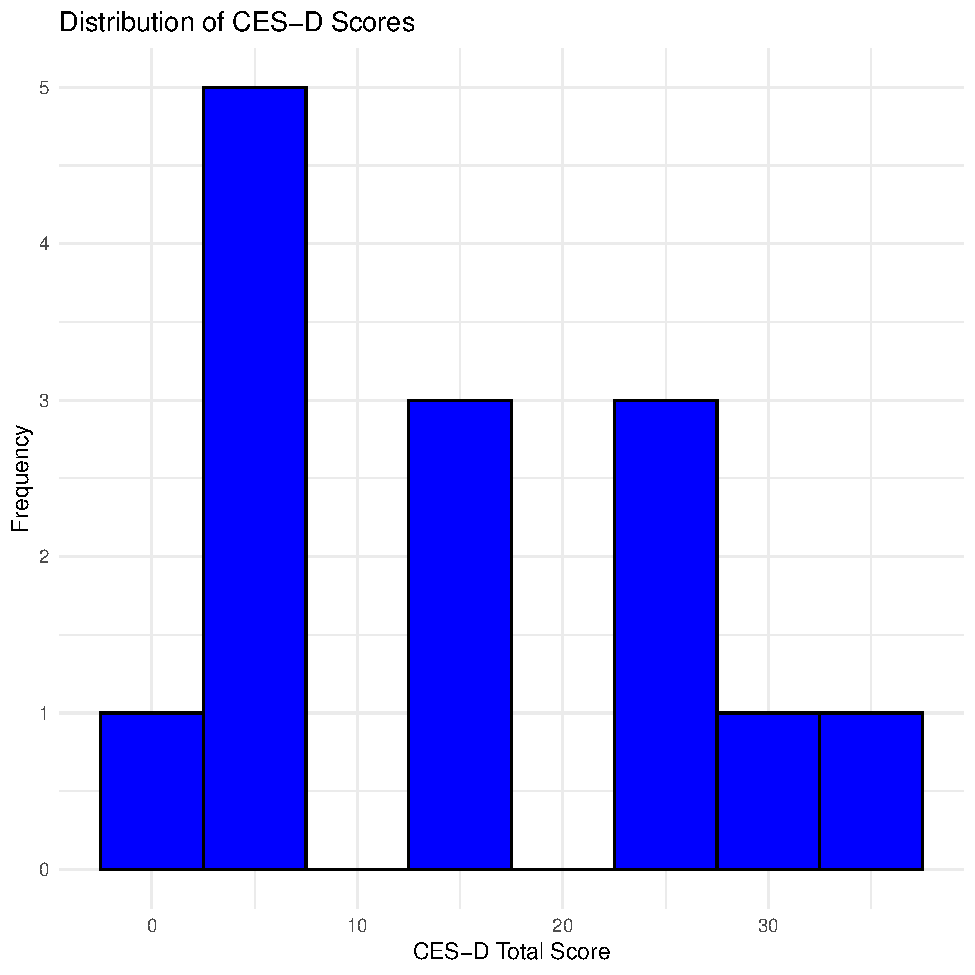
\includegraphics{SE-SCC-Depression_files/figure-pdf/CESD-score-distribution-1.pdf}

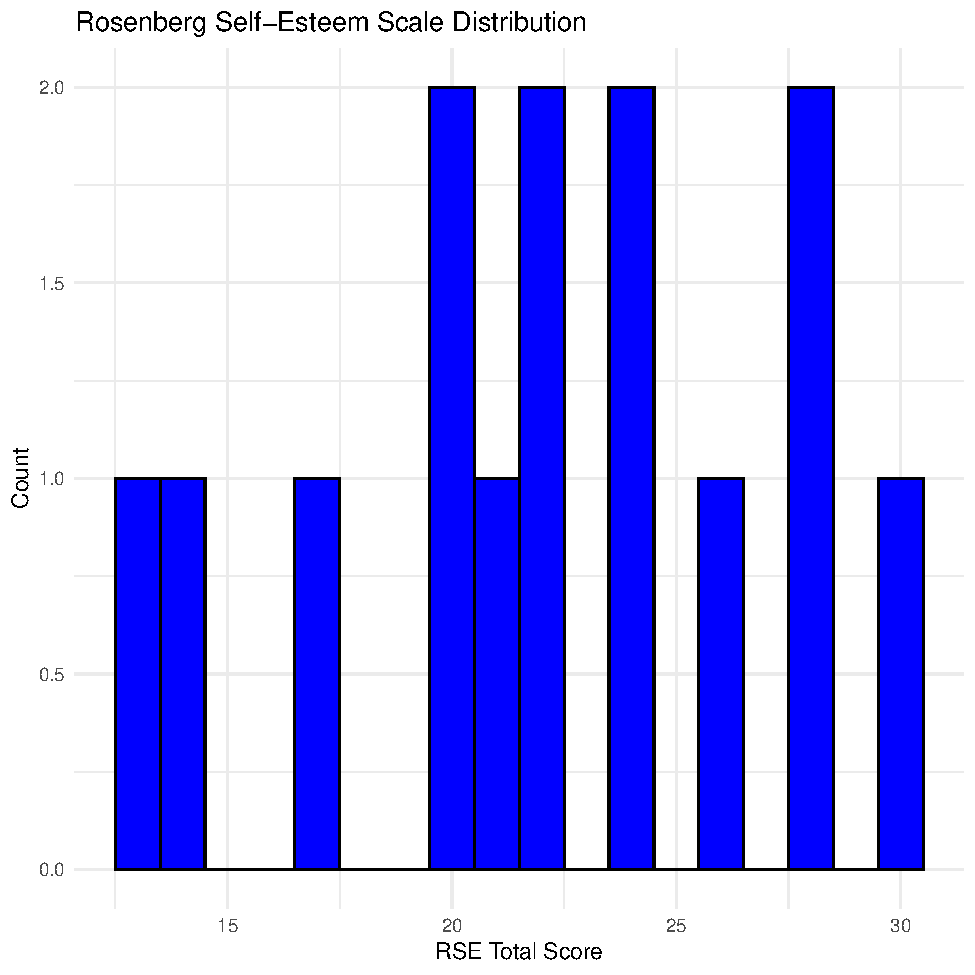
\includegraphics{SE-SCC-Depression_files/figure-pdf/RSES-score-distribution-1.pdf}

\begin{verbatim}
Warning: Removed 2 rows containing non-finite outside the scale range
(`stat_density()`).
\end{verbatim}

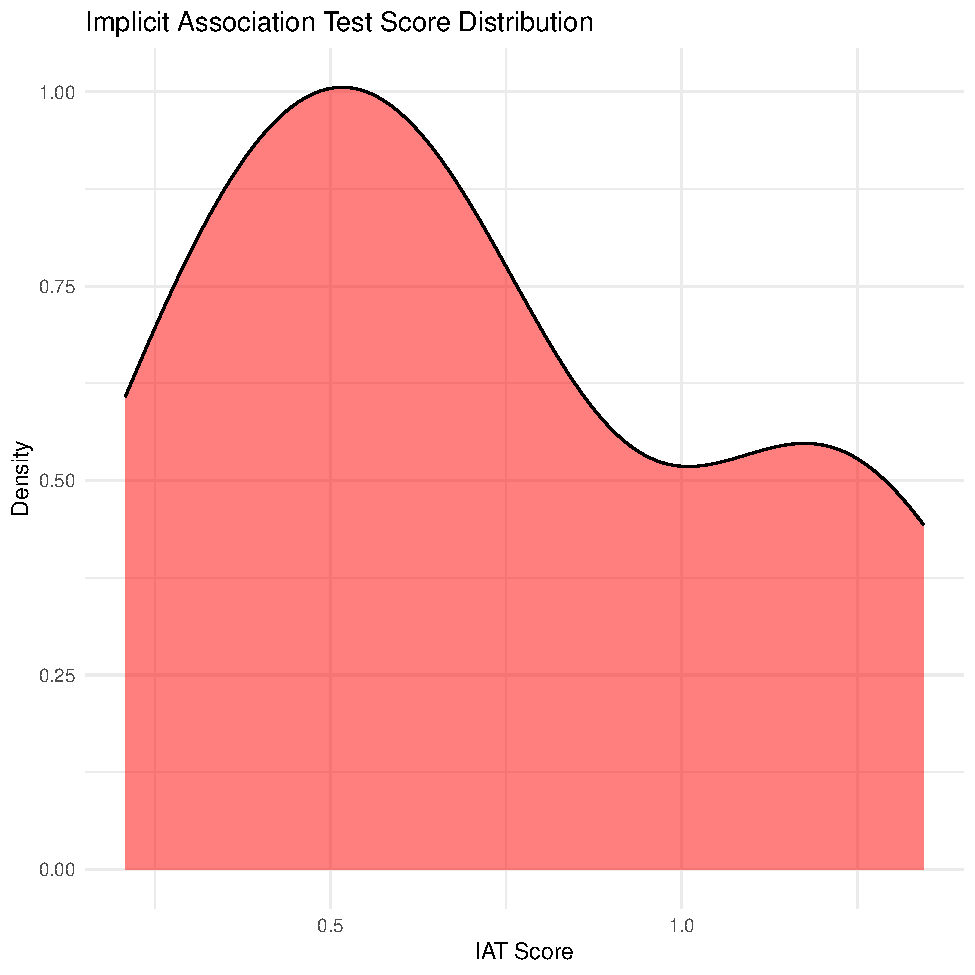
\includegraphics{SE-SCC-Depression_files/figure-pdf/IAT-score-distribution-1.pdf}

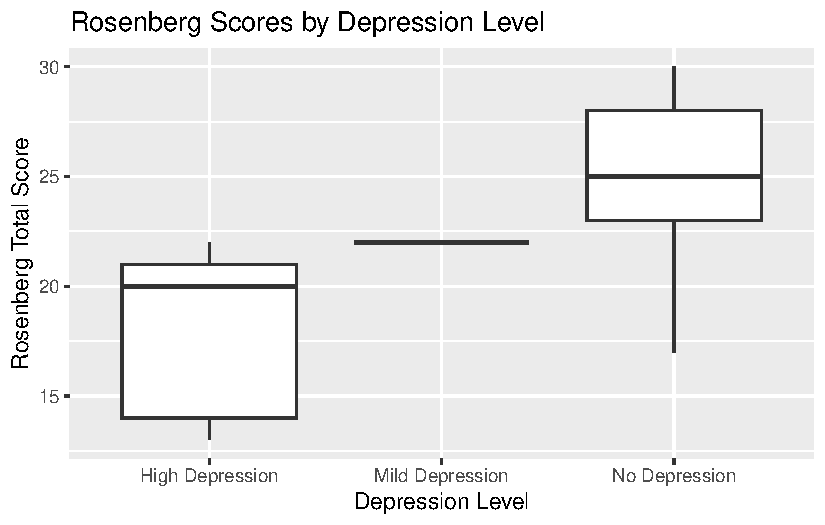
\includegraphics{SE-SCC-Depression_files/figure-pdf/RSES-versus-CESD-level-1.pdf}

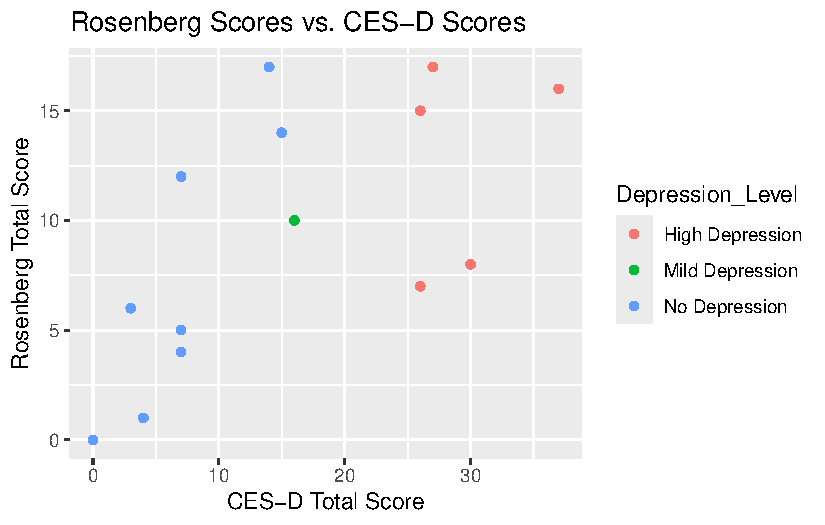
\includegraphics{SE-SCC-Depression_files/figure-pdf/RSES-versus-CESD-total-1.pdf}

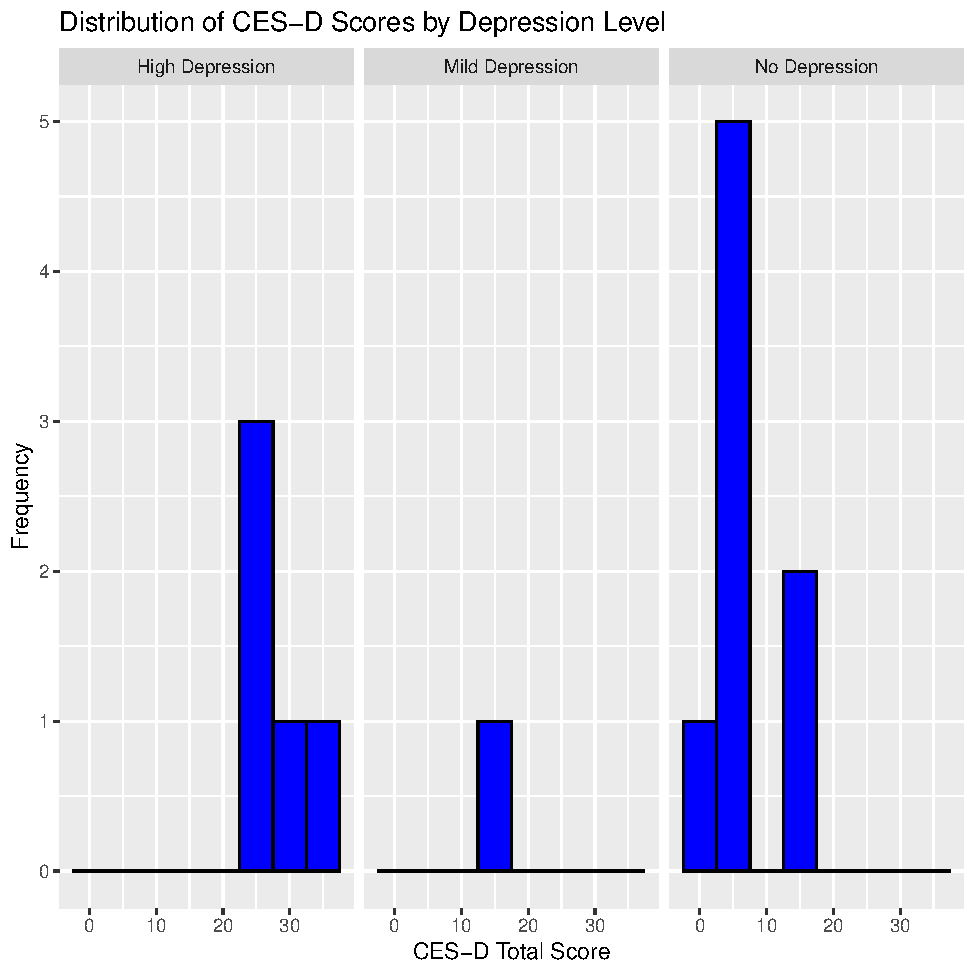
\includegraphics{SE-SCC-Depression_files/figure-pdf/CESD-total-versus-level-1.pdf}

\begin{verbatim}
`geom_smooth()` using formula = 'y ~ x'
\end{verbatim}

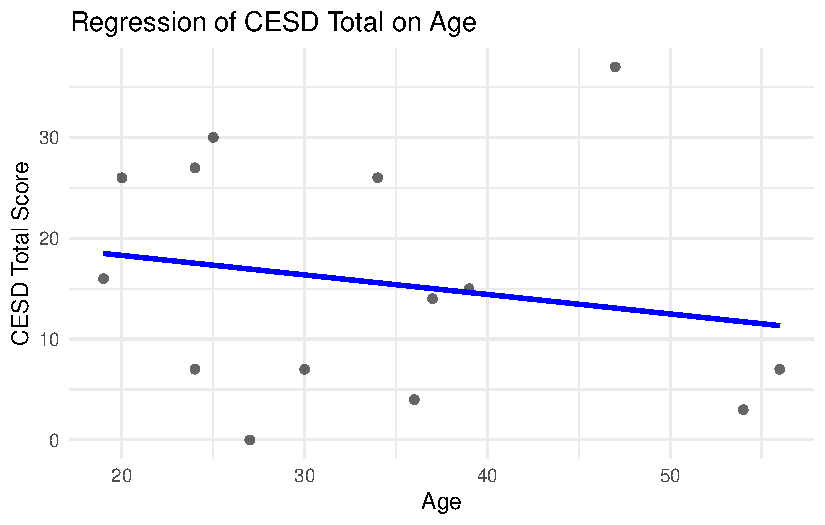
\includegraphics{SE-SCC-Depression_files/figure-pdf/CESD-total-versus-age-1.pdf}

\begin{verbatim}
   Min. 1st Qu.  Median    Mean 3rd Qu.    Max. 
   0.00    7.00   14.50   15.64   26.00   37.00 
\end{verbatim}

\begin{verbatim}

High Depression Mild Depression   No Depression 
              5               1               8 
\end{verbatim}

\begin{verbatim}
                 Df Sum Sq Mean Sq F value   Pr(>F)    
Depression_Level  2 1499.5   749.8   30.14 3.44e-05 ***
Residuals        11  273.7    24.9                     
---
Signif. codes:  0 '***' 0.001 '**' 0.01 '*' 0.05 '.' 0.1 ' ' 1
\end{verbatim}

\begin{verbatim}

Call:
lm(formula = CESD_Total ~ `Demo Q1`, data = wave1_cohort1_clean)

Residuals:
    Min      1Q  Median      3Q     Max 
-16.942  -9.200  -1.749   9.033  23.929 

Coefficients:
            Estimate Std. Error t value Pr(>|t|)  
(Intercept)  22.1689     9.8512    2.25    0.044 *
`Demo Q1`    -0.1936     0.2765   -0.70    0.497  
---
Signif. codes:  0 '***' 0.001 '**' 0.01 '*' 0.05 '.' 0.1 ' ' 1

Residual standard error: 11.92 on 12 degrees of freedom
Multiple R-squared:  0.03924,   Adjusted R-squared:  -0.04083 
F-statistic: 0.4901 on 1 and 12 DF,  p-value: 0.4972
\end{verbatim}

\begin{verbatim}

    Pearson's product-moment correlation

data:  wave1_cohort1_clean$Rosenberg_Total and wave1_cohort1_clean$CESD_Total
t = -3.6003, df = 12, p-value = 0.003644
alternative hypothesis: true correlation is not equal to 0
95 percent confidence interval:
 -0.9051232 -0.3076601
sample estimates:
       cor 
-0.7206088 
\end{verbatim}

\begin{verbatim}
Warning in chisq.test(table(wave1_cohort1_clean$Depression_Level,
wave1_cohort1_clean$Gender)): Chi-squared approximation may be incorrect
\end{verbatim}

\begin{verbatim}

    Pearson's Chi-squared test

data:  table(wave1_cohort1_clean$Depression_Level, wave1_cohort1_clean$Gender)
X-squared = 0.93333, df = 2, p-value = 0.6271
\end{verbatim}

\begin{verbatim}
tibble [14 x 2] (S3: tbl_df/tbl/data.frame)
 $ Depression_Level: chr [1:14] "Mild Depression" "High Depression" "High Depression" "High Depression" ...
 $ Gender          : num [1:14] 0 1 0 1 0 0 1 1 0 1 ...
\end{verbatim}

\begin{verbatim}

High Depression Mild Depression   No Depression 
              5               1               8 
\end{verbatim}

\begin{verbatim}
The mean CES-D score was 15.64286 with a standard deviation of 11.67909 . An ANOVA demonstrated a significant impact of depression level on CES-D scores (F = 30.13599 , p = 3.440381e-05 ). The effect size (Eta-squared) was 0.8456616 .
\end{verbatim}

\begin{verbatim}
# A tibble: 1 x 4
  Mean_CESD SD_CESD Mean_RSE SD_RSE
      <dbl>   <dbl>    <dbl>  <dbl>
1      15.6    11.7     22.1   5.11
\end{verbatim}

``.

\section{Discussion}\label{discussion}

The results suggest a significant relationship between depression and
self-esteem. There was a mean score of 15.6428571in the CES-D,
signifying moderate levels of depressive symptoms present in this
sample. In regards to a relationship between age and depressive
symptoms, a linear regression analysis was performed. This demonstrated
that age was not a significant predictor of depression symptoms
(\emph{β} = -0.1935682, \emph{p} = 0.497248). This demonstrates that age
is not significantly predictive of depressive symptoms in this sample.

This cohort measured:

\begin{itemize}
\item
  Depression
\item
  Implicit Self-Esteem
\item
  Explicit Self-Esteem
\end{itemize}

Future cohorts will also measure:

\begin{itemize}
\tightlist
\item
  Self-Concept Clarity
\end{itemize}

\textbf{only use bold to highlight specific data in a table or figure}

\section{References}\label{references}

\phantomsection\label{refs}
\begin{CSLReferences}{0}{1}
\end{CSLReferences}




\end{document}
